
\section*{1.18 Невалентные взаимодействия, строение соединений с различными типами невалентных взаимодействий}
Невалентные взаимодействия - взаимодействия без образования
новых химических валентных связей. Обычно они меньше 10-20
ккал/моль. \\
Невалентные взаимодействия могут привести либо к
отталкиванию (электронных оболочек), либо к притяжению. \\ 
К притяжению относятся (даны по убыванию
энергии): 
\begin{itemize}
	\item ион-дипольное взаимодействие
	\item водородные связи
	\item диполь-дипольное взаимодействие
	\item мультипольмультипольное взаимодействие
	\item силы Лондона
\end{itemize} 
Большой разброс по энергии имеют комплексы с
переносом заряда (КПЗ). Энергии притяжения много меньше энергий
ионных и ковалентных взаимодействий. Водородные связи
рассматриваются отдельно. \\ \\
\textbf{Ион-дипольное взаимодействие:} \\
	Молекулярный диполь - система из двух равных и
	противоположных по знаку зарядов $+q$ и $-q$, разделённых расстоянием
	$r$. Тогда дипольный момент $p=qr$. Так как ионом создаётся
	электрическое поле, диполь ориентируется к этому иону за счёт
	притяжения разноимённых зарядов. \\ \\
	Формула ион-дипольного взаимодействия:
	\[
	E_{\text{ион-дип}} = const \cdot \dfrac{|z| \cdot \vec{p} \cdot \overline{e}^2}{r^2}
	\]
	где: $const < 0$ (притяжение с выигрышем по инергии), $z$ - величина заряда иона, $\overline{e}$ - заряд электрона,  $\vec{p}=qr$ - дипольный момент, $r$ - расстояние между ионом и диполем. \\ \\
	Так как дипольный момент является малой величиной, энергия
	ион-дипольного взаимодействия меньше энергии ион-ионного
	взаимодействия. Более того, энергия ион-дипольного
	взаимодействия квадратично убывает с расстоянием, а ионионного - обратно пропорционально:
	\[
	E_{\text{ион-ион}} = const \cdot \dfrac{z^+ \cdot z^- \cdot \overline{e}^2 }{r^2}
	\]
	Такое взаимодействие проявляется при сольватации, когда идёт
	взаимодействие иона с полярной молекулой растворителя. При
	растворении наблюдается очень много таких взаимодействий,
	поэтому энергия сольватации может превысить высокую энергию
	кристаллической решетки, и соединения растворится.  \\ \\
	При этом становится очень важна среда, в которой осуществляется
	то или иное превращение. \\ \\
	\textbf{Диполь-дипольное взаимодействие:} \\
	Крайние случаи взаимодействия диполей:
	
\begin{wrapfigure}{r}{0.15\textwidth}
	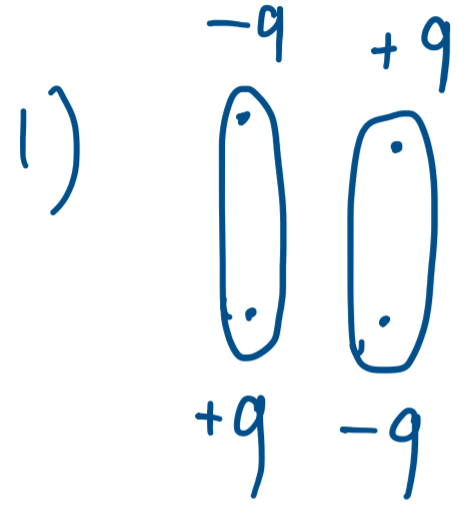
\includegraphics[width=0.15\textwidth]{rr}
\end{wrapfigure}
1) Заряды компенсируются, суммарный дипольный момент равен нулю. 
\\\\\\\\\ \\

\begin{wrapfigure}{l}{0.15\textwidth}
	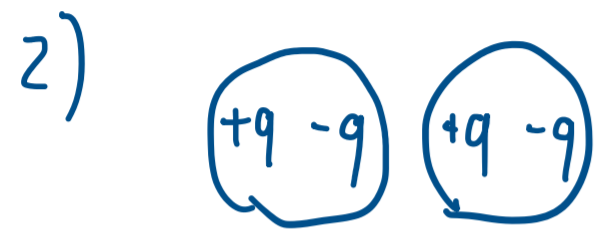
\includegraphics[width=0.15\textwidth]{rr2}
\end{wrapfigure}
2) Расстояние между некомпенсированными зарядами увеличится, суммарный дипольный момент увеличится. \\ \\ 
Энергии обоих вариантов будут одинаковы, если диаметры эллипса
(в условном изображении диполя) относятся, как 1.12:1
\begin{figure} [H]
	\centering {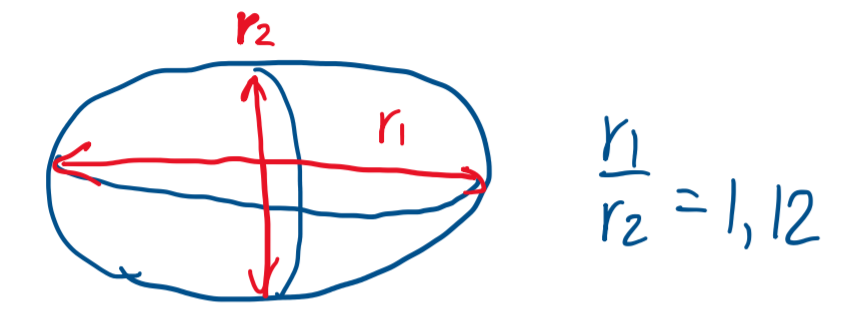
\includegraphics[scale=0.5]{rr3}}
\end{figure}
	\[
	E_{\text{дип-дип}} = const \cdot \dfrac{\vec{p_1}	 \cdot \vec{p_2} }{r^3}
	\]
	Энергия диполь-дипольного взаимодействия убывает с
	расстоянием ещё быстрее, чем энергия ион-дипольного
	вазимодействия. Энергия диполь-дипольного вазимодействия
	невелика, лежит в диапазоне 2.5-5 кДж/моль. \\ \\
	Диполь-дипольные взаимодействия хорошо проявляются при
	низких температурах, при температурах порядка комнатной и выше
	ими можно пренебречь из-за беспорядочного движения молекул. \\ \\ 
	Такое взаимодействие проявляется в таких полярных жидкостях,
	как вода и фтороводород. \\ \\ 
\textbf{Дисперсионное взаимодействие:} \\
Силы Лондона (дисперсионные взаимодействия) - самые слабые.
Их также не очень корректно называют Ван-дер-ваальсовыми
силами (так как зачастую под ним подразумевают и дипольдипольные взаимодействия, и другие). \\ \\
За счёт этого взаимодействия в жидком или твердом состоянии
удерживаются неполярные молекулы (водород, азот, кислород и
т.д.). 
	\[
	E_{\text{дисп}} = const \cdot \dfrac{2 \cdot \vec{p_1}	 \cdot \vec{p_2} }{r^6}
	\]	
\begin{figure} [H]
	\centering {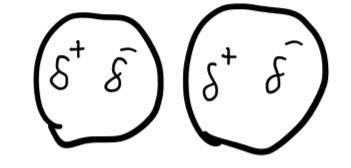
\includegraphics[scale=0.5]{rr4}}
\end{figure}
где $\vec{p_1}, \vec{p_2}$ - мгновенные согласованные диполи. \\
Так как дипольные моменты маленькие, а в знаменателе - шестая
степень, то ничтожные изменения расстояний приводят к
разрушению этих взаимодействий. \\ \\
Фрагмент кристаллической структуры твёрдого хлора:
\begin{figure} [H]
	\centering {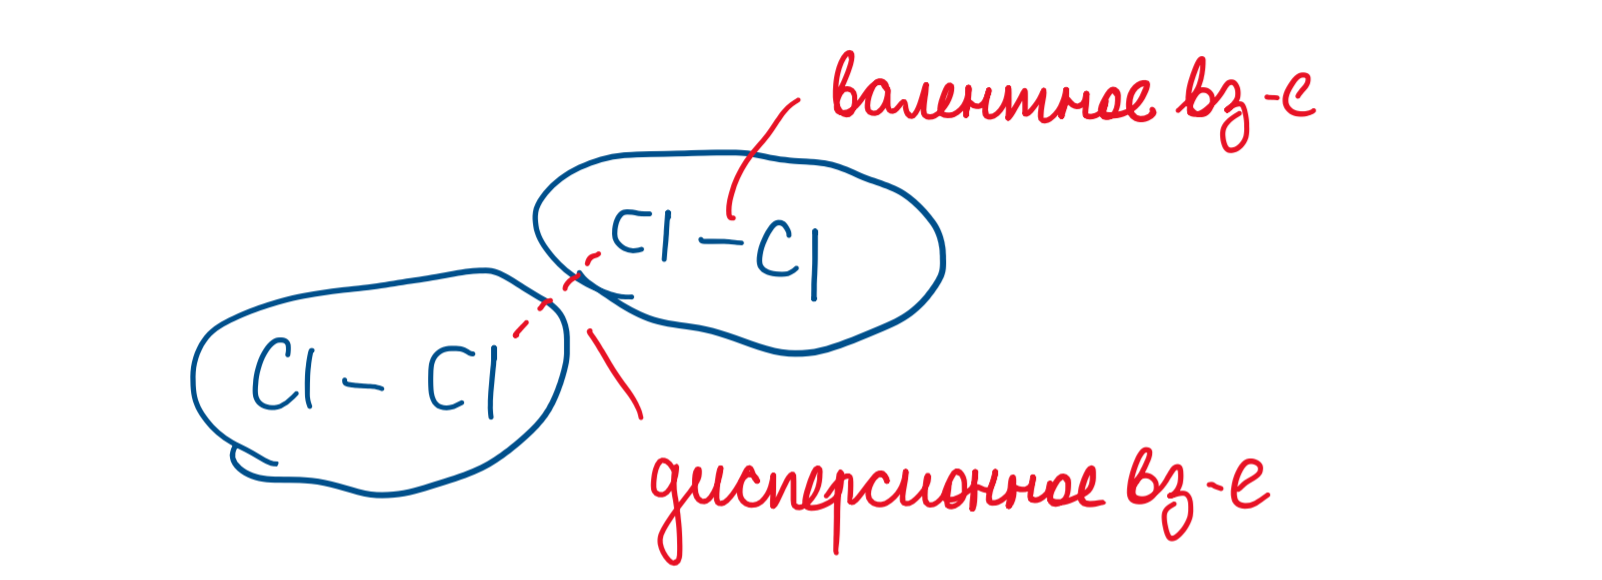
\includegraphics[scale=0.5]{rr5}}
\end{figure}
Величина дисперсионного взаимодействия тут примерно в 10 раз
меньше величины валентного взаимодействия атомов хлора, но всё
равно величина довольно значимая, пренебрегать не стоит. \\ \\
Но, например, для $Li_2$ формула выше неприменима: константа
получится очень большая; при конденсации будут не молекулы, а
кристаллическая решётка. \\ \\
Из расстояния между молекулами в молекулярных кристаллах
вычисляют Ван-дер-ваальсовы радиусы. \\ \\
\textbf{Отталкивание молекул:} \\
При определенном расстоянии между молекулами очень резко
увеличивается, то есть, начинается отталкивание - молекулы
просто не могут подойти ближе. Два атома практически
невозможно вдавить друг в друга. \\ \\
Зависимость энергии взаимодействия молекул от расстояния:
\begin{figure} [H]
	\centering {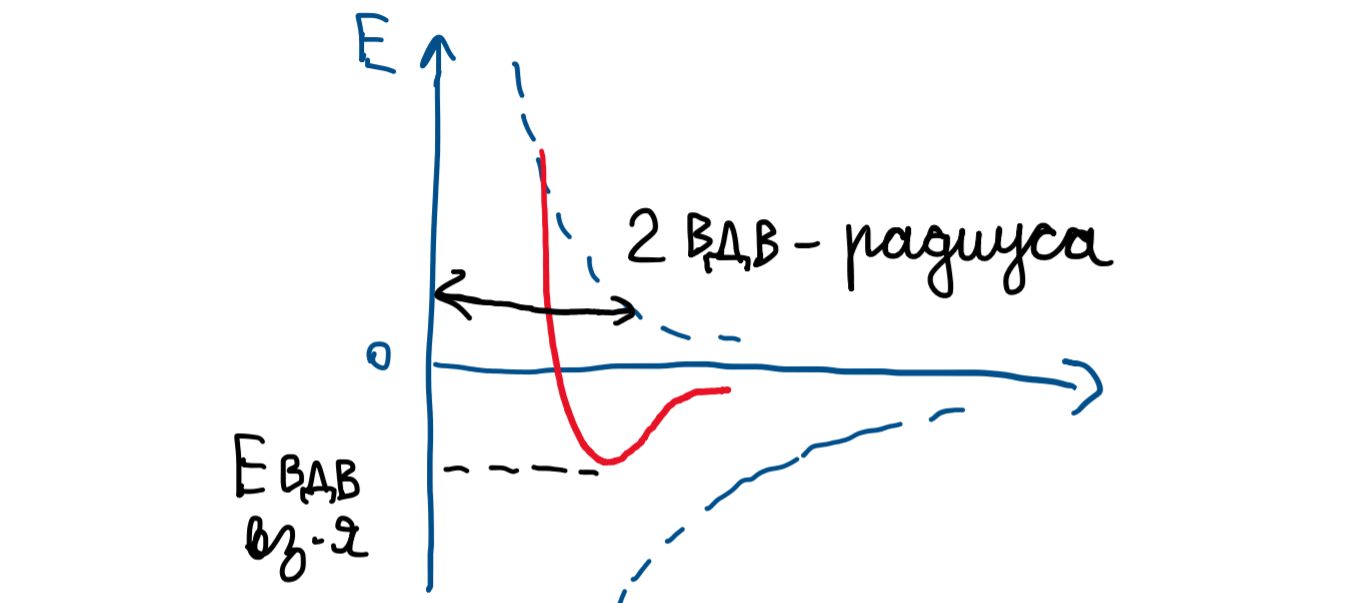
\includegraphics[scale=0.5]{rr6}}
\end{figure}
Заметим, что для атомов водорода в молекуле воды расстояние
между ними значительно меньше, чем два их Ван-дер-ваальсовых
радиуса. То есть, валентные оболочки атомов водорода «вдавлены»
друг в друга. \\ \\
Есть примеры и у углеводородов: расстояния между первым и
третьим атомом в бензоле и противоположными атомами в
циклобутане меньше их двух Ван-дер-ваальсовых радиусов.
\begin{figure} [H]
	\centering {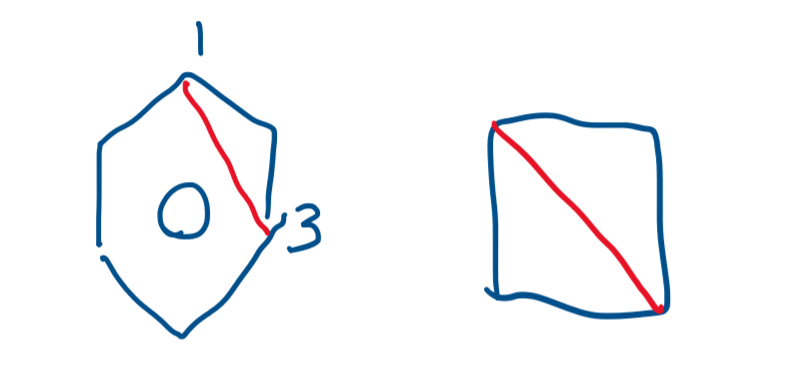
\includegraphics[scale=0.5]{rr7}}
\end{figure}
Энергия отталкивания задаётся выражением:
\[
E_{\text{отталкивания}} = K \cdot r^{-n}, \quad K > 0, n = 5 - 12 \text{ (чаще всего 12)}
\]
Большой показатель степени в знаменателе говорит о том, что при
столкновении молекулы встречают практически твёрдую стенку. \\ \\
\textbf{Комплексы с переносом заряда:} \\
Это можно рассмотреть, как самое слабое донорно-акцепторное
взаимодействие. Эти комплексы очень слабы. Они имеют
небольшой энергетический зазор между связывающей и
разрыхляющей МО (их энергии очень слабо отличаются от
орбитали донора и орбитали акцептора => выигрыш ничтожный),
поэтому спектр поглощения такого комплекса лежит в видимой
области спектра. \\ \\
Посмотрим на реакцию:
\begin{figure} [H]
	\centering {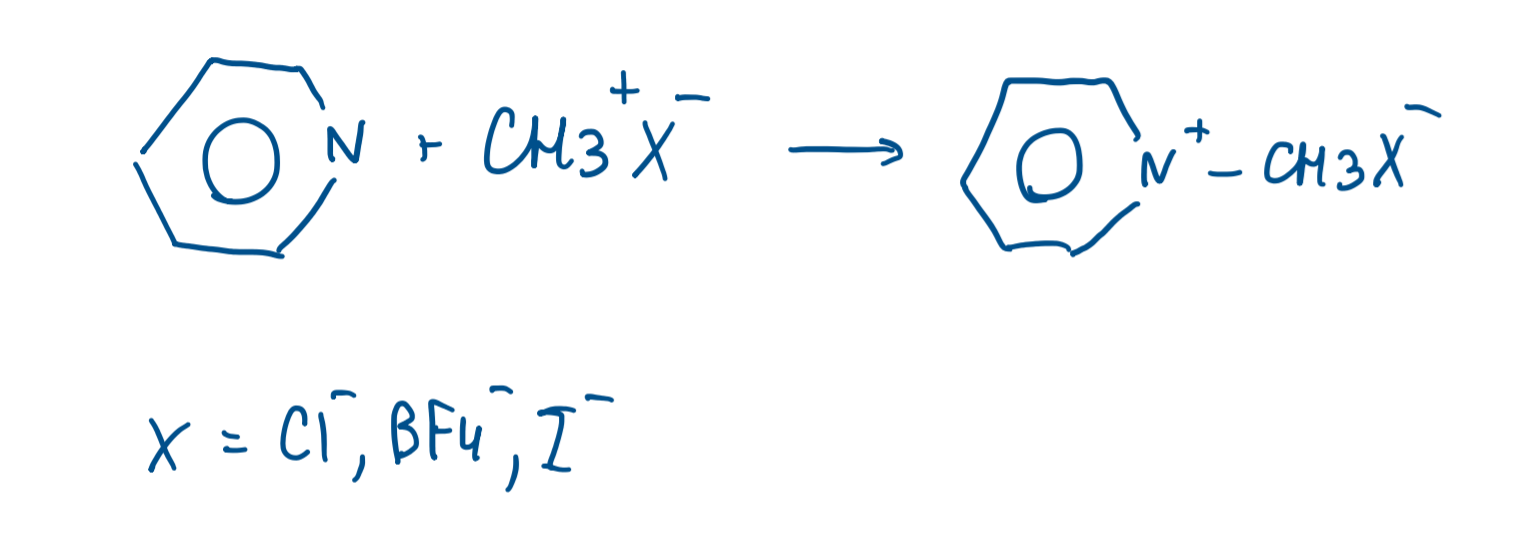
\includegraphics[scale=0.5]{rr8}}
\end{figure}
Все соли, кроме $X=I^-$, бесцветны. Соль с иодидом окрашена, потому
что возникает КПЗ, где анион иода выступает донором, а
акцептором - $\pi$ орбиталь $PyCH_3^+$. \\ \\
Другие примеры КПЗ: диоксан дибромид, $I_3^-$, иод в спирте и в
бензоле.


\section*{1.19 Строение соединений переходных металлов в высших и низших степенях окисления. Изомерия комплексных соединений.}
Все переходные металлы являются типичными металлами, атомы способны легко окисляться и быть в положительном валентном состоянии, есть много соединений, где валентное состояние считается нулевым.
Общая характеристика:
\begin{itemize}
	\item Существуют координационные соединения и комплексы
	\item $E_{\text{связи}}$ при движении вниз растёт
	\item Высокая ЭО среди металлов
	\item $d$-оболочка хорошо поляризуема 
	\item Самые распространенные степени окисления: $+2$, $+3$
	\item Большая устойчивость соединений тяжелых $d$-металлов в высших степенях окисления
	\item $4d$ и $5d$ элементы имеют большие координационные числа, чем $3d$ элементы
\end{itemize}
\begin{figure} [H]
	\centering {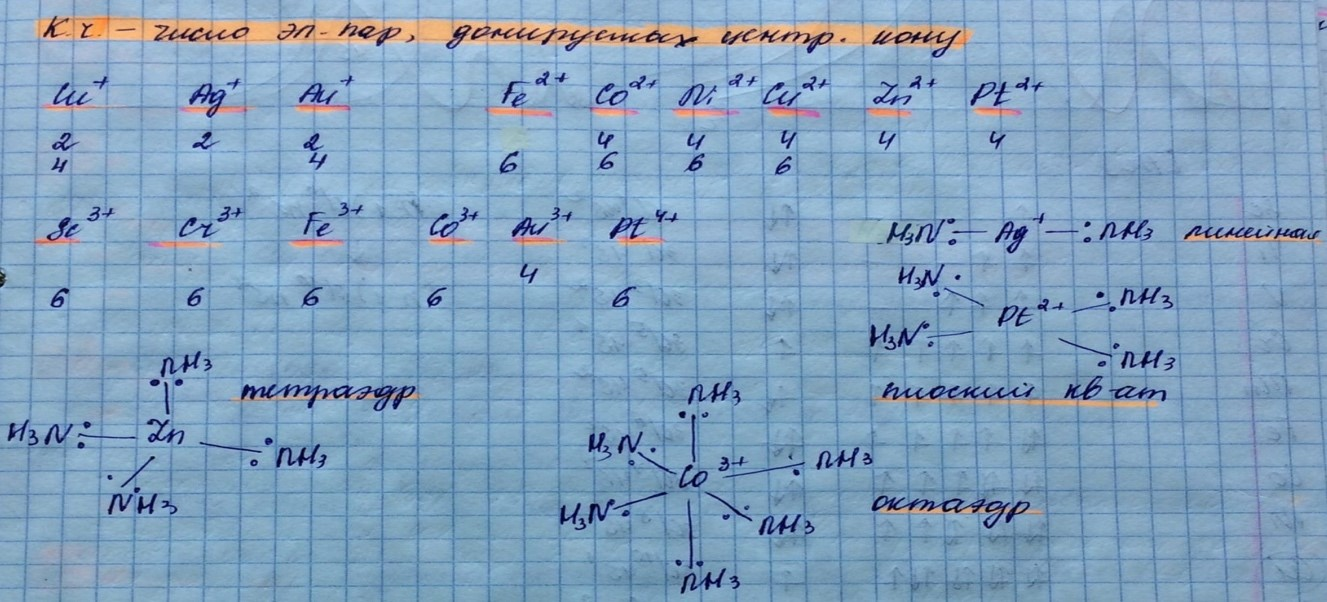
\includegraphics[scale=1.2]{qq1}}
\end{figure}
Электронные конфигурации:
\begin{figure} [H]
	\centering {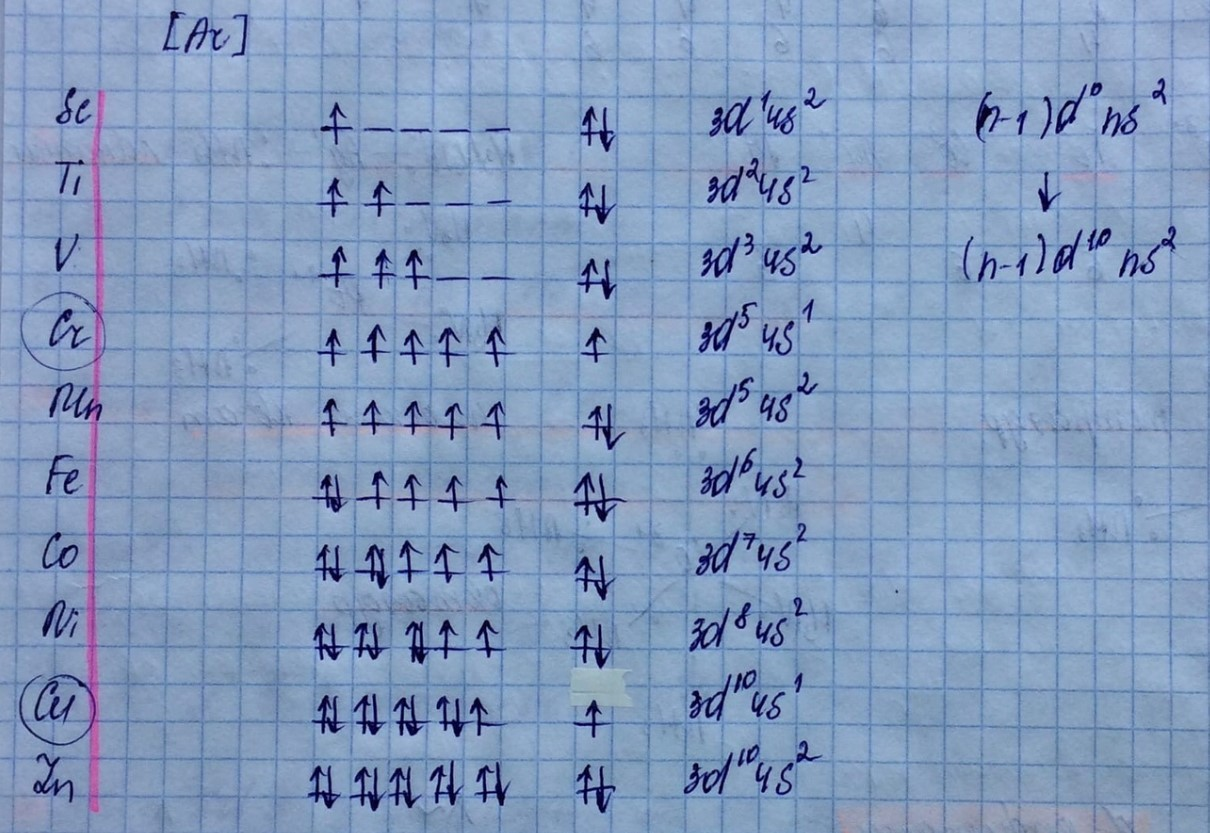
\includegraphics[scale=0.8]{qq2}}
\end{figure}
Возможно образование четкого октаэдрического поля.  
\[
M^{2+} + 6H_2O = \left[M(H_2O)_6\right]^{2+}
\]
Отсюда и происходит термин «кристаллическое поле». 
\begin{figure} [H]
	\centering {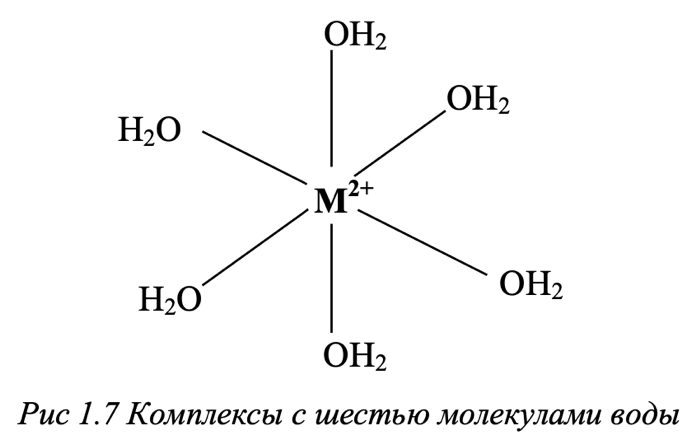
\includegraphics[scale=0.9]{qq3}}
\end{figure}
Если вокруг металла четыре лиганда, кристаллические поля могут быть в форме квадрата или тетраэдра. Если шесть, то кристаллическое поле октаэдрическое, такие соединения больше всего распространены. 
\begin{figure} [H]
	\centering {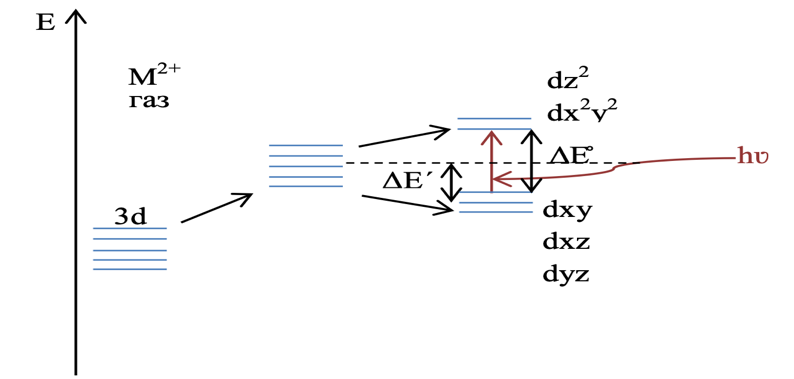
\includegraphics[scale=1.5]{qq4}}
\end{figure}
Происходит расщепление $d$ орбитали на две группы: три орбитали уходят вниз, а две – вверх. Центр тяжести остается на месте. Вниз уходят $d_{xy}$, $d_{xz}$, $d_{yz}$, те, которые между лигандами. \\
Вверх уходят $d_{z^2}$, $d_{x^2 -y^2}$. Если электронов не много, они все должны оказаться внизу. $\Delta E$ - общее расщепление, связано с тем, насколько сильно лиганды поляризуют. Некоторые лиганды расщепляют слабее, некоторые - сильнее (согласно стереохимическому ряду).
\begin{flushleft}
	\begin{figure} [H]
	\centering {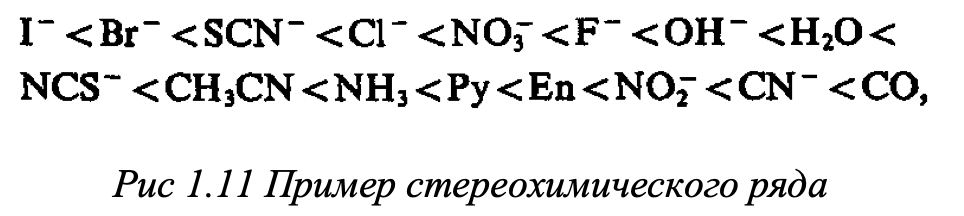
\includegraphics[scale=1]{qq5}}
\end{figure}
\end{flushleft}
\textbf{Изомерия комплексных соединений:} \\
\begin{itemize}
	\item Ионизационная изомерия: \\
	Темно-красное $\left[Co(NH_3)_5 Br \right]SO_4$ и красное $\left[Co(NH_3)_5SO_4 \right]Br$ при диссоциации в воде дают различные анионы: первое - $SO^{2-}_4$, второе - $Br^-$
	\item Cольватная (гидратная) изомерия: \\ 
	Осуществляется при участии нейтральных молекул растворителя и заключается в перераспределении их молекул между внутренней и внешней сферой комплексного соединения. Например три изомера гидратированного хлорида хрома:
	\begin{itemize}
		\item серо-голубой $\left[ Cr(H_2O)_6Cl_3  \right] $ 
		\item светло-зеленый $\left[ Cr(H_2O)_5Cl  \right]Cl_2 \cdot H_2O$ 
		\item темно-зеленый цис-$\left[ Cr(H_2O)_4Cl_2  \right]Cl \cdot 2H_2O$ 
	\end{itemize}
	\item Координационная изомерия: \\
	 Характерна для соединений с комплексными катионами и анионами и проявляется во взаимном обмене лигандами между катионами и анионами. \\
	 Примерами являются:
	 \begin{itemize}
	 	\item $\left[ Co(NH_3)_6  \right] \left[ Cr^{III}(CN_6)\right]$ и $\left[ Cr(NH_3)_6  \right] \left[ Co^{III}(CN_6)\right]$
	 	\item $\left[ Cu(NH_3)_4  \right] \left[ PtCl_4\right]$ (фиолетовый) и $\left[ Pt(NH_3)_4  \right] \left[ CuCl_4\right]$ (зеленый)
	 \end{itemize}
	\item Проявление амбидентатности: \\
	Этот тип изомерии обусловлен наличием лигандов, способных образовывать связи через разные донорные атомы (такие лиганды называют амбидентатными). Например красный и желтый изомеры комплекса $ \left[ Co(NH_3)_5(NO_2) \right]Cl_2 $ причем в первом из них лиганд $NO_2^-$ координирован через атом кислорода ($Co-ONO^-$, нитрито-комплекс), а во втором через атом азота ($Co-NO_2^-$, нитро-комплекс).
	\item Оптическая изомерия: \\
	Она связана с явлением оптической активности некоторых соединений - вращением плоскости поляризации света. \\
	Основным условием наличия оптической изомерии является ассиметричное строение химического соединения. \\
	По сравнению с октаэдрическими, тетраэдрические комплексы имеют оптические изомеры только в случае четырех лигандов разной природы. В настоящее время получены многочисленные оптические изомеры моно- и полиядерных комплексов. \\ Оптически активные комплексы называют хиральными, а оптические изомеры - энантиомерами.
	\begin{figure} [H]
		\centering {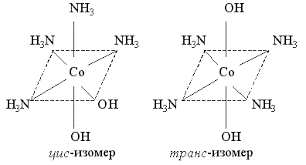
\includegraphics[scale=1.2]{qq6}}
	\end{figure}
\end{itemize}

\section*{1.20 Соединения переходных металлов 4 группы. Геометрия молекул в зависимости от природы лигандов, их электронное строение, способы получения и химическое поведение.}
\begin{itemize}
	\item $Ti$: $(+2), +3, +4$ \quad координационное число $6$ \quad $3d^24s^2$
	\item $Zr$: $(+2), +3, +4$ \quad координационные числа $7, 8$ \quad $4d^2 5s^2$
	\item $Hf$: $(+3), +4$ \quad координационные числа $7, 8$ \quad $4f^4 5d^2 6s^2$
\end{itemize}
\ul{Координационное число $6$}
\[
\left[TiF_6 \right]^{2-} \quad \left[Ti(H_2O)_6 \right]^{3+} \quad \left[TiCl_6 \right]^{3-} \quad \text{ октаэдр.}
\]
$d^1$, эффект Яна-Теллера:
\begin{figure} [H]
	\centering {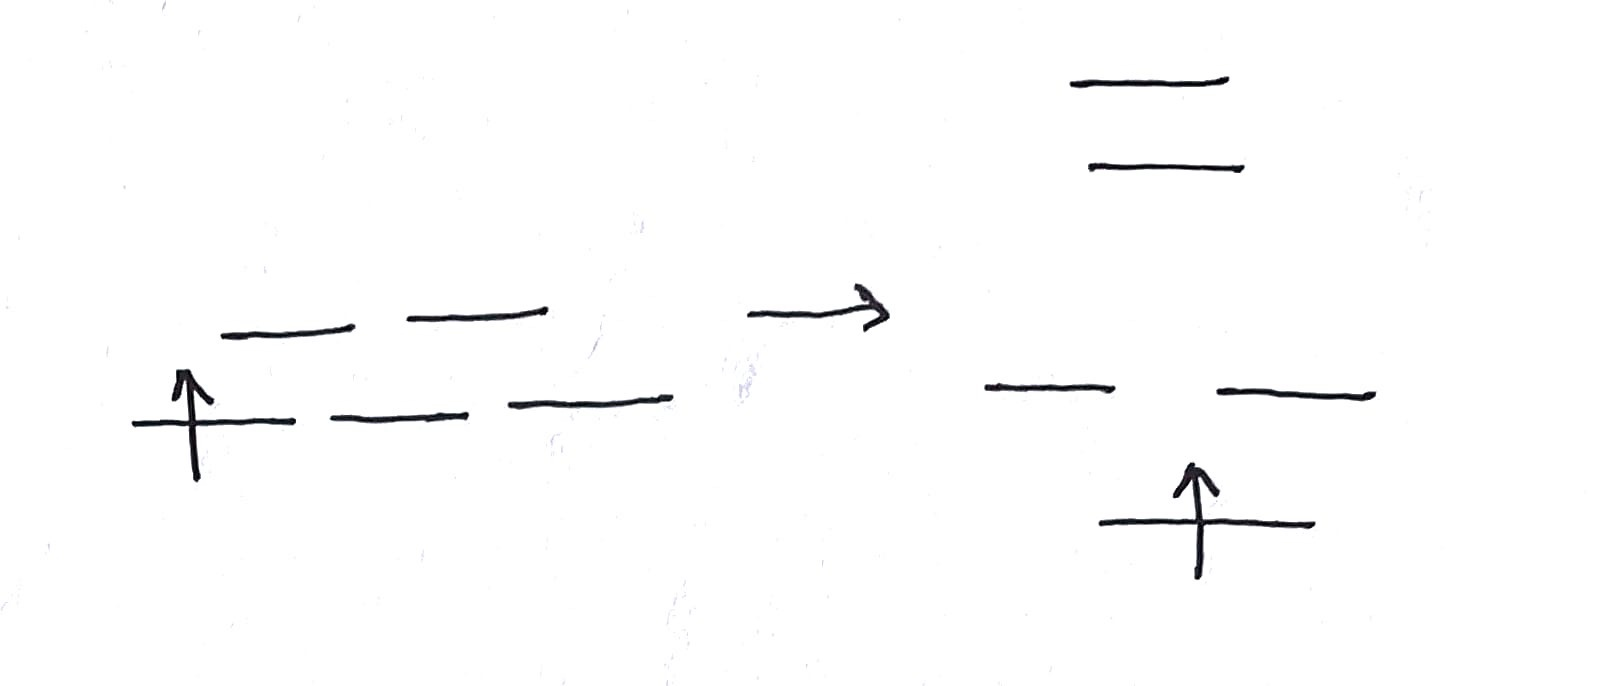
\includegraphics[scale=0.2]{aaq}}
\end{figure}
\textbf{Степень окисления $+3$} \\
$Ti^{+3}$ - восстановитель (с $KMnO_4, H_2O$) \\
$Ti$ в степени окисления $+4$ не образует устойчивых комплексов (ЭСКП $= 0$) \\
$ \left[ZrF_6 \right]^{2-} $ (КЧ = $6$)
\textbf{Степень окисления $+4$} \\
Соли титанила:
\begin{figure} [H]
	\centering {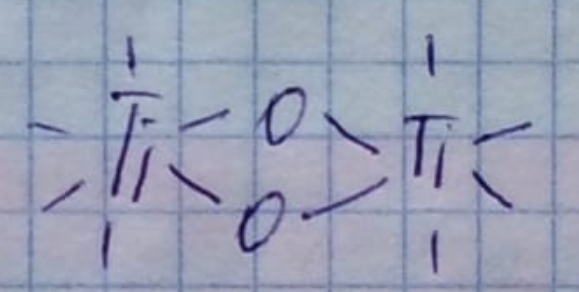
\includegraphics[scale=0.5]{aa1}}
\end{figure}
$d^0$ \\
\ul{Координационное число $7$}: $ \left[Zr^{+4}F_7 \right]^{3-} \quad \left[Hf^{+4}F_7 \right]^{3-} $ \\
\ul{Координационное число $8$}: $ \left[Zr^{+4}(ox)_4 \right]^{4-} \quad \left[Zr^{+4}(acac)_4 \right]^{4-} $ \\
\ul{Координационное число $4$}: $ \left[Hf(NPh_2)_4 \right] \quad \left[Zr(NPh_2)_4 \right] $ - стабилизируется объемными $L$ \\ \\
В природе:
\begin{itemize}
	\item рутил $TiO_2$
	\item циркон $ZrSiO_4$
	\item $Hf$ не образует собственных минералов
\end{itemize}
\begin{figure} [H]
	\centering {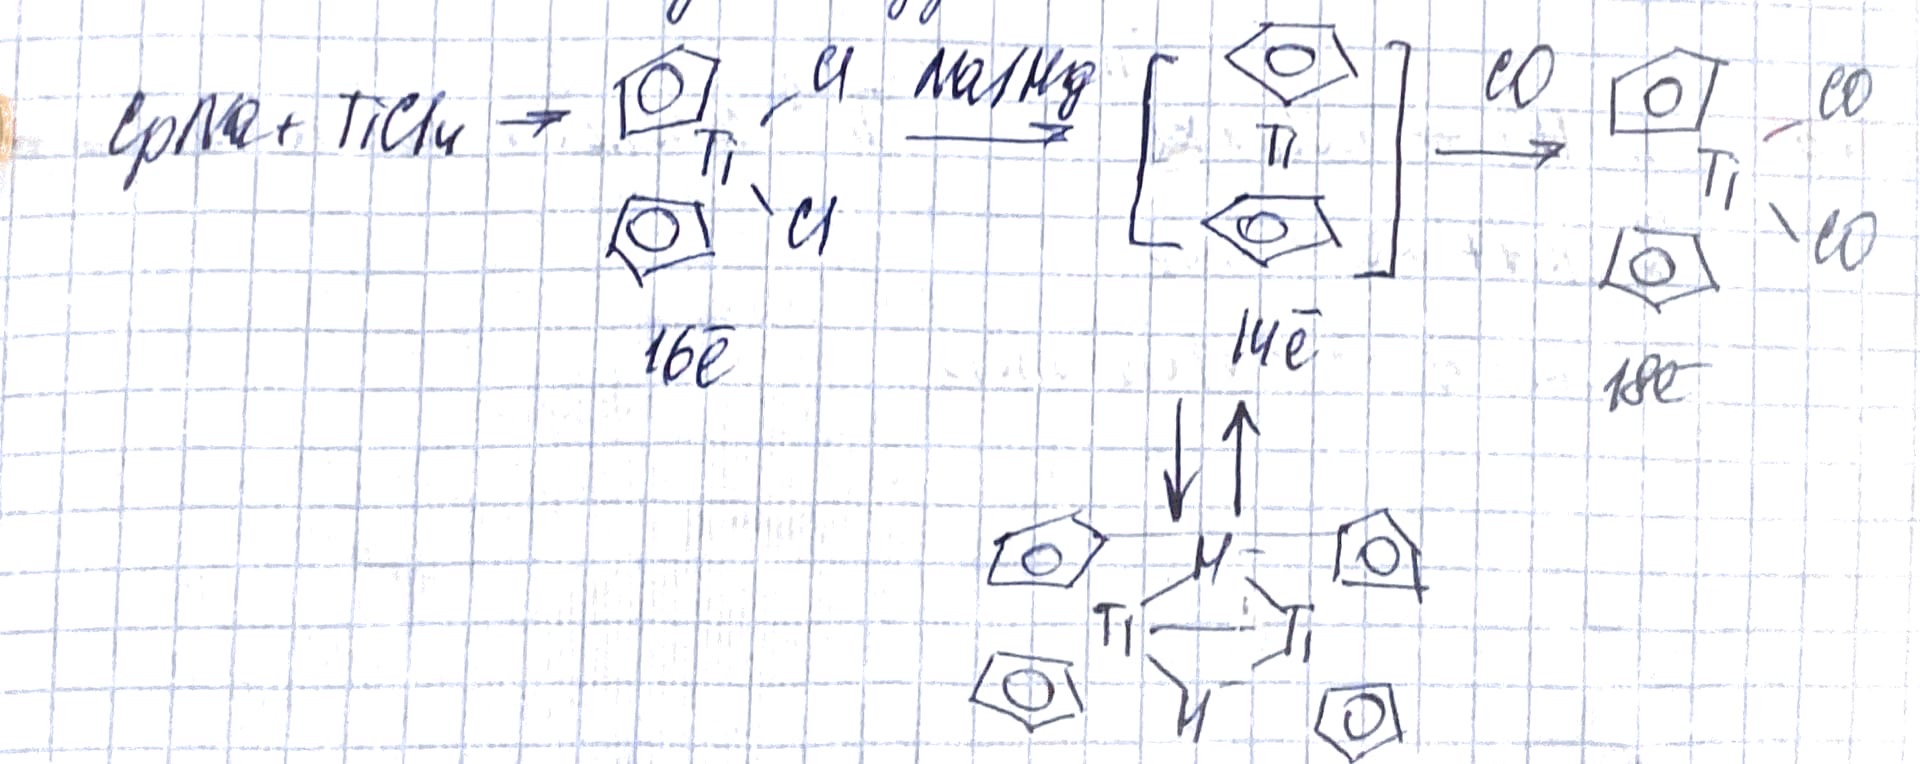
\includegraphics[scale=0.25]{aa2}}
\end{figure}
$Ti$: \\ 
\begin{itemize}
	\item Вскрытие руды
	\item $TiCl_4 + 2 Mg = Ti + 2MgCl_2$
	\item Очистка: $TiI_4 = Ti + 2I_2$
\end{itemize}
$Zr$: \\ 
\begin{itemize}
	\item Вскрытие минералов
	\item $ZrOSO_4 + 4 KF + 2HF = K_2\left[ZrF_6 \right] + H_2O + K_2SO_4$
	\item $K_2\left[ZrF_6 \right] + 4Na = Zr + 4NaF + 2KF$
	\item Очистка: $ZrI_4 = Zr + 2I_2$
\end{itemize}
Свойства:
\begin{itemize}
	\item $Ti$:
	\begin{itemize}
		\item $+ HCl = 2TiCl_3 + H_2$
		\item $+ KOH + H_2O = K_2TiO_3 + H_2 $
		\item $+ HF = H_2\left[TiF_6 \right] + H_2 $
		\item $+ Cl_2 = TiCl_4 $
		\item $+ HNO_3(\text{к}) = TiO_2 \cdot H_2O + NO_2 + H_2O $		
	\end{itemize}
	\item $Zr, Hf$:
	\begin{itemize}
		\item $+ HCl \not = $
		\item $+ KOH \not = $
		\item $+ HF \not = $
		\item $+ Cl_2 = ZrCl_2$
		\item $+ HNO_3(\text{к}) + HF  = H_2\left[ZrF_6 \right] + NO + H_2O $		
	\end{itemize}
\end{itemize}
\textbf{Степень окисления $+3$} 
\begin{align*}
Ti + HCl &= TiCl_3 + H_2 \quad \text{ $Ti^{+3}$ - сильный восстановитель, слабый окислителль}\\
ZrCl_4 + Zr &= ZrCl_3 \\
HfCl_4 + Al &= t = HfCl_3 + AlCl_3 
\end{align*}	
\textbf{Степень окисления $+4$} \\
Свойства: \\
$TiO_2$:
\begin{itemize}
	\item $+ C + Cl_2 = TiCl_4 + CO$
	\item $+ KOH = K_2TiO_3 + H_2 $
	\item $+ KH_2 = K_2TiF_6$
	\item $+ nH_2O = TiO(OH)_2 + H_2O	$	
\end{itemize}
Две формы существования титановой кислоты $TiO_2 \cdot 2H_2O$:
\begin{figure} [H]
	\centering {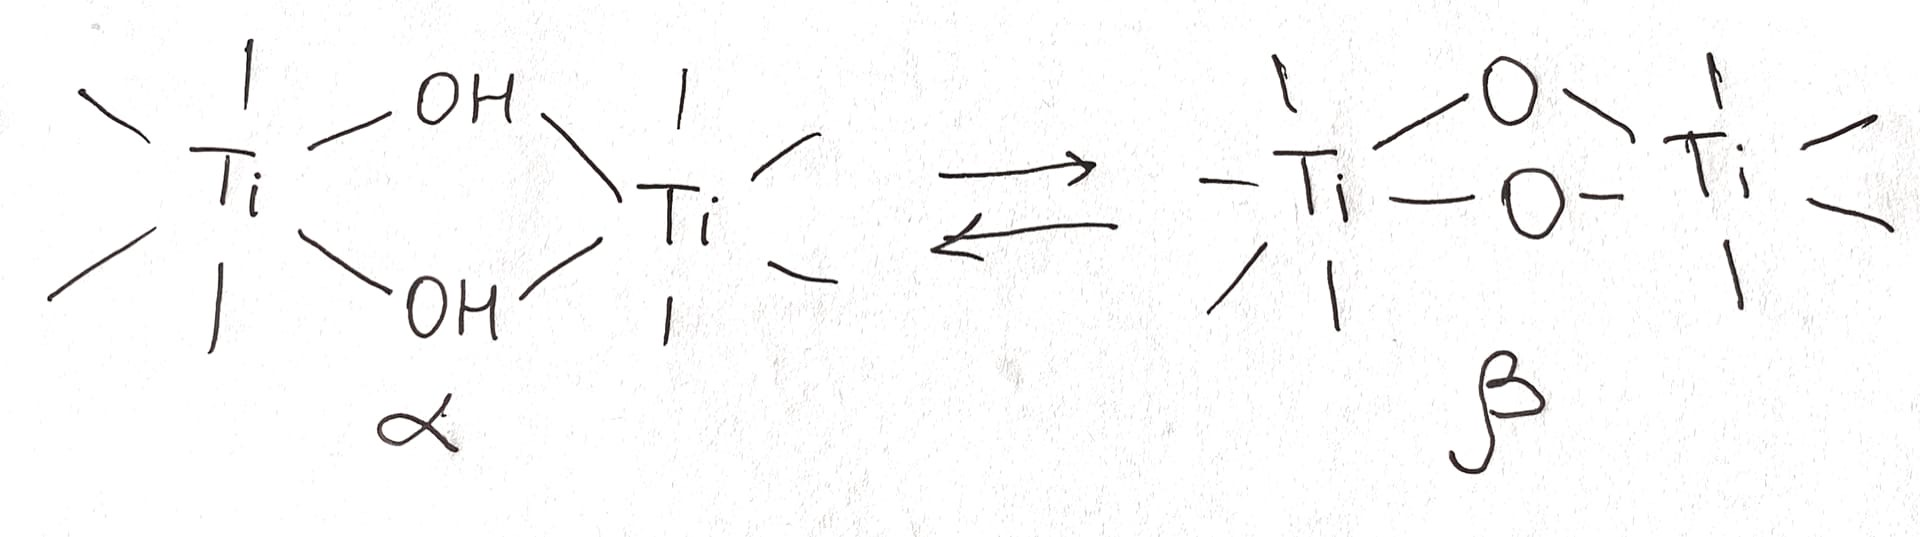
\includegraphics[scale=0.25]{aa3}}
\end{figure}
$TiCl_4$:
\begin{itemize}
	\item $+ H_2O + NaOH =TiO(OH)_2 $
	\item $+ H_2 = TiCl_3 + HCl$	
\end{itemize}
\section*{1.21 Соединения переходных металлов 5 группы. Геометрия молекул в зависимости от природы лигандов, их электронное строение, способы получения и химическое поведение.}
\begin{itemize}
	\item $V$: $(+2), +3, +4, +5$ \quad $3d^34s^2$
	\item $Nb$: $(+2), (+3), (+4), +5$ \quad $4d^3 5s^2$
	\item $Ta$: $(+3), (+4), +5$ \quad $4f^{14} 5d^3 6s^2$
\end{itemize}
$V$:
\begin{itemize}
	\item $2(NH_4)_3VO_4 = t = V_2O_5 + 6 NH_3 + 3 H_2O$
	\item $V_2O_5 + 5 Ca = 5CaO + 2V$
\end{itemize}
$Ta, Nb$:
\begin{itemize}
	\item Вскрытие минералов, разделение
	\item Восстановление:
	\begin{align*}
		K_2(TaF_7) + 5 Na &= Ta + 2KF + 5 NaF \\
		Nb_2O_5 + 5C &= 2Nb + 5CO
	\end{align*}
\end{itemize}
Свойства:
\begin{itemize}
	\item $V$:
	\begin{itemize}
		\item $+ F_2 = VF_5$
		\item $+ KOH \not = $
		\item $+ O_2 = V_2O_5 $
		\item $+ HF = H_3\left[VF_6 \right] $
		\item $+ HNO_3(\text{к}) = VO_2NO_3 + NO_2 + H_2O$	
		\item $+ H_2SO_4 (\text{к}) = VO_SO_4 + SO_2 + H_2O  $
		\item $+ Br_2(I_2) = VBr_3(VI_3) $
		\item $+ Cl_2 = VCl_4 $	
	\end{itemize}
	\item $Nb, Ta$:
	\begin{itemize}
		\item $+ KOH \not = $
		\item $+ O_2 = Nb_2O_5 $
		\item $+ HF \not =  $
		\item $+ HNO_3(\text{к}) + HF = H_2\left[NbF_7 \right] + NO + H_2O $	
		\item $+ Cl_2 = NbCl_5 $		
	\end{itemize}
\end{itemize}
\textbf{Степень окисления $+2, +3$} ($d^3$) - основные свойства \\
$VaCl_3  + H_2 = VCl_2 + HCl$ \\
$NaVO_3 = Na/Hg, HCl = VCl_2 + NaCl + Hg + H_2O$ \\
Известны все $VHal_3$: $VF_3$ - н/р, остальные: $VCl_3 + H_2O = \left[V(H_2O)_6 \right]^{3+} + Cl^-  $ 
Восстановители:
\begin{align*}
VSO_4 + H_2SO_4 &= V_2(SO_4)_3 + H_2 \\	
VCl_3 + KMnO_4 + KOH &= KVO_3 + MnO_2 + KCl + H_2O 
\end{align*}
$V^{+3}, d^2$ - октаэдрические комплексы: $ \left[VCl_3(THF)_3 \right], \left[V_6 \right]^{3-}, \left[V(CO)_6 \right] $ \\
$V^{+2}, d^3$ - октаэдрические комплексы, в р-ре $ \left[V(H_2O)_6 \right]^{2+}, \left[V(CN)_6 \right]^{4-}, \left[V(phen)_3 \right]Cl_2 $ \\
\textbf{Степень окисления $+4$} - амфотерные свойства \\
$VO_2$ - структура рутила
\begin{align*}
NaVO_3 + N_2H_4 + H_2SO_4 &= VOSO_4 + N_2 + Na_2SO_4 + H_2O \\
V_2O_5 + H_2C_2O_4 &= t = VO_2 + CO_2 + H_2O
\end{align*}
Ванадильные комплексы:
\begin{figure} [H]
	\centering {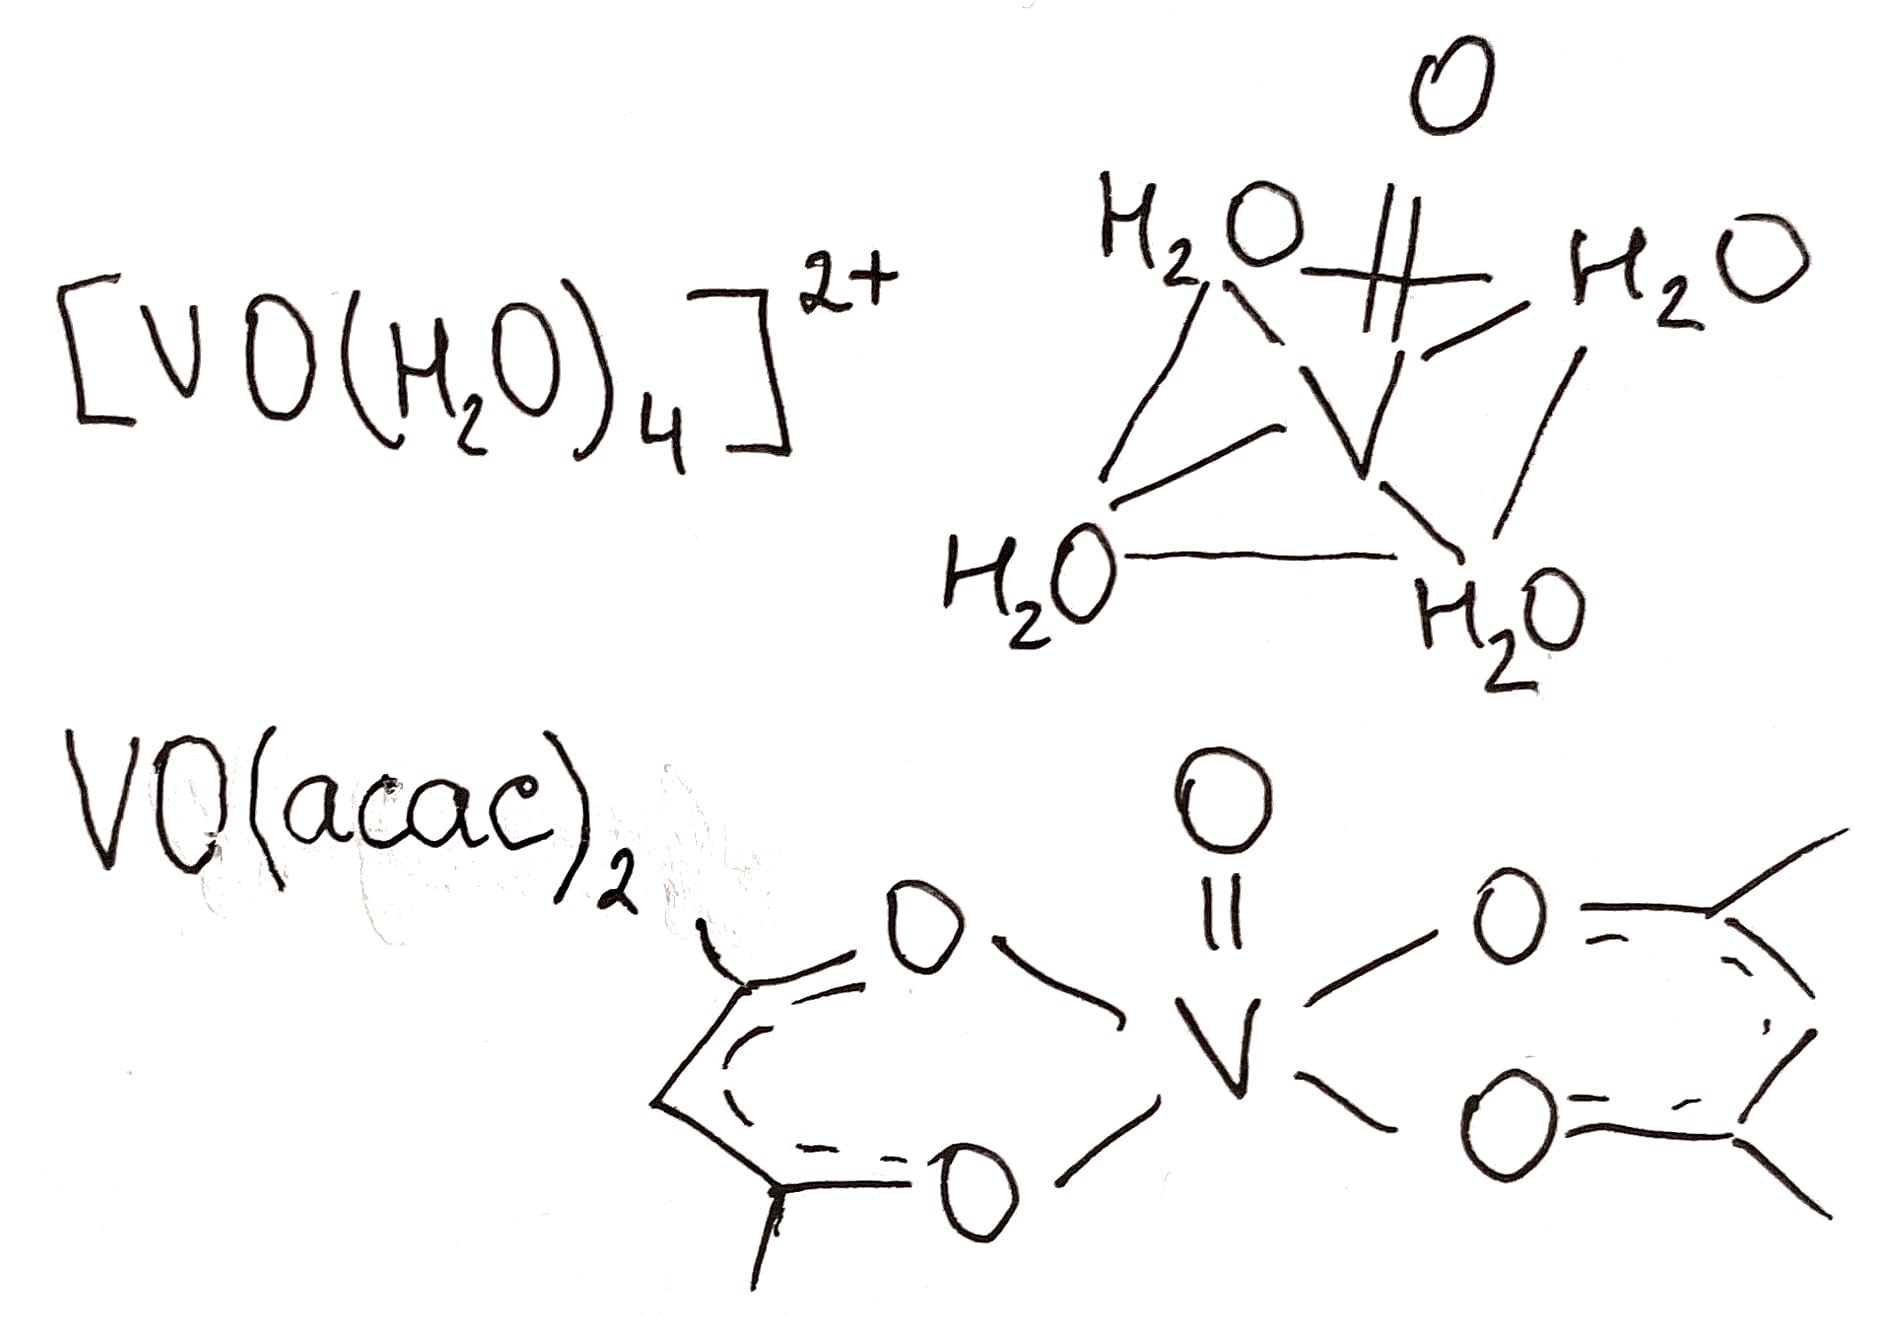
\includegraphics[scale=0.15]{ee1}}
\end{figure}
С $N-$донорными $L$: $(NH_4)_2\left[VOCl_4 \right]$ \\
$\left[VF_6 \right]^{2-}$ - октаэдр \\
$ 	\left[Nb(CN)_8 \right]^{4-}, \left[Nb(ox)_4 \right]^{4-} $ \\
\textbf{Степень окисления $+5$} - $V_2O_5$ - амфотерные свойства \\
В растворах $V^{+5}$ проявляет окислительные свойства \\
Гидролиз солей: $ NbCl_5 + H_2O = Nb_2O_5 \cdot H_2O + HCl $
Кислоты Льюиса: 
\begin{align*}
TaF_5 + BrF_3 &= \left[Br_2F_2 \right]\left[TaF_6 \right] \\
NbF_6 + KF &=   K_2\left[NbF_7 \right]
\end{align*}
$V^{+5}$ образует изо- и гетерополисоединения. \\
$VO_4^{3-}$ - тетраэдры \\
\[
\left[TaF_8 \right]^{3-} \quad \left[TaCl_5(bipy) \right] \quad \left[NbOCl_4 \right]
\] 
Фторидные комплексные анионы: $ \left[NbF_7 \right]^{2-}, \left[NbF_8 \right]^{3-} $ \\
В низших степенях окисления $Nb$ и $Ta$ образуют треугольные кластеры состава $M_3X_8$, октаэдрические кластеры $M_6X_{12}$
\section*{1.22 Соединения переходных металлов 6 группы. Геометрия молекул в зависимости от природы лигандов, их электронное строение, способы получения и химическое поведение.}
\begin{itemize}
	\item $Cr$: $+2, +3, (+4), (+5), +6$ \quad \quad $3d^54s^1$
	\item $Mo$: $+2, +3, +4, +5, +6$ \quad $4d^1 5s^1$
	\item $W$: $(+2), (+3), (+4), +5, +6$ \quad $4f^{14} 5d^4 6s^2$
\end{itemize}
Свойства:
\begin{itemize}
	\item $Cr$:
	\begin{itemize}
		\item $+ H_2SO_4 (\text{к})/HNO_3(\text{к}) = Cr_2(SO_4)_3 / Cr(NO_3)_3 + SO_4/NO_2 + H_2O $
		\item $+ KNO_3, KOH \text{(расплав)} = K_2CrO_4 + KNO_3 + H_2O$
		\item $+ HCl = CrCl_2 + H_2$
		\item $+ KOH \not =$
		\item $+ H_2O \text{(пар)} = Cr_2O_3 + H_2$	
		\item $+ O_2 = Cr_2O_3$
		\item $+ Hal = CrHal_3 $
		\item $+ S, \,\, P, \,\, N_2, \,\, C, \,\, As, \,\, B = CrS, \,\, CrP_2, \,\, CrN,\,\, Cr_7C_3, \,\, CrAs,\,\, CrB $	
	\end{itemize}
	\item $Mo, W$:
	\begin{itemize}
		\item $+$ кислоты неок. $ \not = $
		\item $+ Hal = MoF_6, \,\, WCl_6 \,\, MoCl_5 \,\, WBr_5 $
		\item $+ O_2 = MoO_3$
		\item $+ HNO_3 + HF/HCl = H_2\left[WF_8 \right]/MoO_2Cl_2 + NO_2/NO + H_2O $		
	\end{itemize}
\end{itemize}
$Cr$: хромистый железняк $FeCr_2O_4$
\[
FeCr_2O_4 + 4C = Fe + 2Cr + 4CO \text{ (феррохром)}
\]
\begin{itemize}
	\item Вскрытие минерала
	\item $Cr_2O_3 + 2 Al = Al_2O_3 + 2 Cr$ (технический хром)
\end{itemize}
$Mo$: молибденит $MoS_2$
\begin{align*}
MoS_2 + O_2 &= MoO_3 + SO_2 \\
MoO_3 + H_2 &= Mo + H_2O
\end{align*}
$W$: вольфрамит $(Fe, Mn)WO_4$
\begin{itemize}
	\item Вскрытие минерала
	\item $WO_3 + 3 H_2 =W + 3 H_2O$
\end{itemize}
\textbf{Степень окисления $+2, +3$} - $Mo, W$ низкие с.о.\\
Для $Mo, W$ мало монноядерных комплексов, много с $M-M$, в основном кластеры. \\
$d^3$- окт.: $ \left[Mo^{+3}(H_2O)_6 \right]^{3+} \quad \left[Mo^{+3}(HCOO)_6 \right]^{3-} \quad \left[Mo^{+3}(HPO_4)_4 \right]^{2-}$ \\ 
$\left[Mo^{+3}(SCN)_6 \right]^{3-} \quad \left[Mo^{+3}Cl_6 \right]^{3-} \quad \left[W_2^{+3}Cl_9 \right]^{3-} $ \\
$ WCl_2 + 2Cl_2 = CCl_4 = W_6Cl_{16} $ \\
$ MoO_3 + 9CO = Mo(CO)_6 + 3CO_2 $
\textbf{Степень окисления $+2, +3$} - $Cr^{2+}$ - сильный восстановитель: \\
$CrCl_2 + 2 NaCp = Cr(Cp)_2 + 2 NaCl$ \\
$d^4$, эффект Яна-Теллера: $ \left[CrHal_3 \right]^{-} \quad \left[CrHal_4 \right]^{2-} \quad \left[Cr(H_2O)_6 \right]^{2+}  $
\textbf{Степень окисления $0$} - $Cr$ \\
\begin{align*}
CrCl_3 + Al + CO &= THF = Cr(CO)_6 + AlCl_3 \\
CrCl_3 + Al + 2C_6H_6 &= Cr(C_6H_6)_2 + AlCl_3
\end{align*}
\textbf{Степень окисления $+3$} - $Cr^{+3}$ - амфортерные свойства \\
$Cr_2O_3 + HNO_3 / KOH \not = $ - химически инертный \\
$Cr_2O_3 + KOH + KNO_3 = t = K_2CrO_4 + KNO_2 + H_2O$ \\
Много комплексов: инертны и устойчивы \\
\[
\left[Cr(H_2O)_6 \right]^{3+} \quad \left[CrCl(H_2O)_5 \right]^{2+} \quad \left[Cr(acac)_3 \right] \quad \left[Cr(ox)_3 \right]^{3-} \quad \left[Cr(CN)_6 \right]^{3-}	
\]
$d^3$, нет эффекта Яна-Теллера \\
Окислитель: $ CrCl_3 + Zn = CrCl_2 + ZnCl_2 $ \\
Восстановитель: $ Cr_2(SO_4)3 + MnO_2 + H_2O = H_2CrO_4 + MnSO_4 $ \\ 
\textbf{Степень окисления $+4, +5$} \\
$MoO_2, WO_2$ - искаженная структура рутила \\
$ \left[MoCl_6 \right]^{2-} \quad \left[Mo(CN)_8 \right]^{4-} \quad \left[W_3O_2(OAc)_6(H_2O)_3\right]^{2-} \text{(хелатный)} $ \\
$ \left[MoCl_3L_2 \right] $ где $L = THF, PEt_3,  bpy$ \\
$\left[MoOCl_5 \right]^{2-}$ устойчивы галогениды и оксогалогениды \\
$CrF_5$ - тригональная бипирамида \\
$CrF_4$ - тетраэдр \\
\textbf{Степень окисления $+6$} - $Cr^{+6}$ - окислитель (самая устойчивая с.о.)\\
$CrO_3 + 2KOH = K_2CrO_4 + H_2O$ \\ 
Хроматы сильные окислители в кислоте и слабые в щелочи. \\
$\left[CrO_4\right]^{2-}  $ - тетраэдр \\
$ Cr_2O_3 $ - цепочка из тетраэдров \\
$Mo^{+6}, W^{+6}$ - плохие окислители \\
Полимеризация \\
$\left[MoO_4\right]^{2-} \quad \left[WO_4\right]^{2-} $ - тетраэдры \\
$Cr$ и $Mo$ в степени окисления $+6$ и $W$ в степени окисления $+5$ образуют изо- и гетерополисоединения (анионы Кеггина, молибденовый синий)

\section*{1.23 Соединения переходных металлов 7 группы. Геометрия молекул в зависимости от природы лигандов, их электронное строение, способы получения и химическое поведение.}
\begin{itemize}
	\item $Mn$: $(+1), +2, +3, +4, (+5), +6, +7$	
	\item $Tc$: $(+2), +3, +4, +5, (+6), +7$
	\item $Re$: $(+2), +3, +4, +5, +6, +7$
\end{itemize}
В природе 
\begin{itemize}
	\item $Mn$: \\
	$MnO \cdot nH_2O$ - пиролюзит, $MnCO_3$ - родохрозит, $Mn_2O_3 \cdot nH_2O$ - манганат.
	\item $Tc$: \\
	нет стабильных изотопов
	\item $Re$: \\
	редкий и рассеянный  элемент, извлекается из молибденовых руд
\end{itemize}
Свойства:
\begin{itemize}
	\item $Mn$:
	\begin{itemize}
		\item $+ N_2 = Mn_3N_2 $
		\item $+ H_2O = Mn(OH)_2 + H_2 $
		\item $+ HCl = MnCl_2 + H_2 $
		\item $+ KOH \not =  $
		\item $+ H_2 \not = $
		\item $+ F_2  = MnF_3$
		\item $+ O_2 = Mn_3O_4 $
		\item $+ C = Mn_3C \quad Mn_7C_3 \quad Mn_5C_2 $
		\item $+ Cl_2 =  MnCl_2 $		
	\end{itemize}
\end{itemize}
$Mn^0$ расстворяется с образованием комплексов:
\begin{align*}
Mn + 6 NaCN + \frac12 O_2 + H_2O &= Na_4\left[Mn^{+2}(CN)_6\right] + 2NaOH \\
Mn + 6 NaCN + H_2O &= Na_5\left[Mn^{+1}(CN)_6\right] + NaOH + \dfrac12 H_2
\end{align*}
\begin{figure} [H]
	\centering {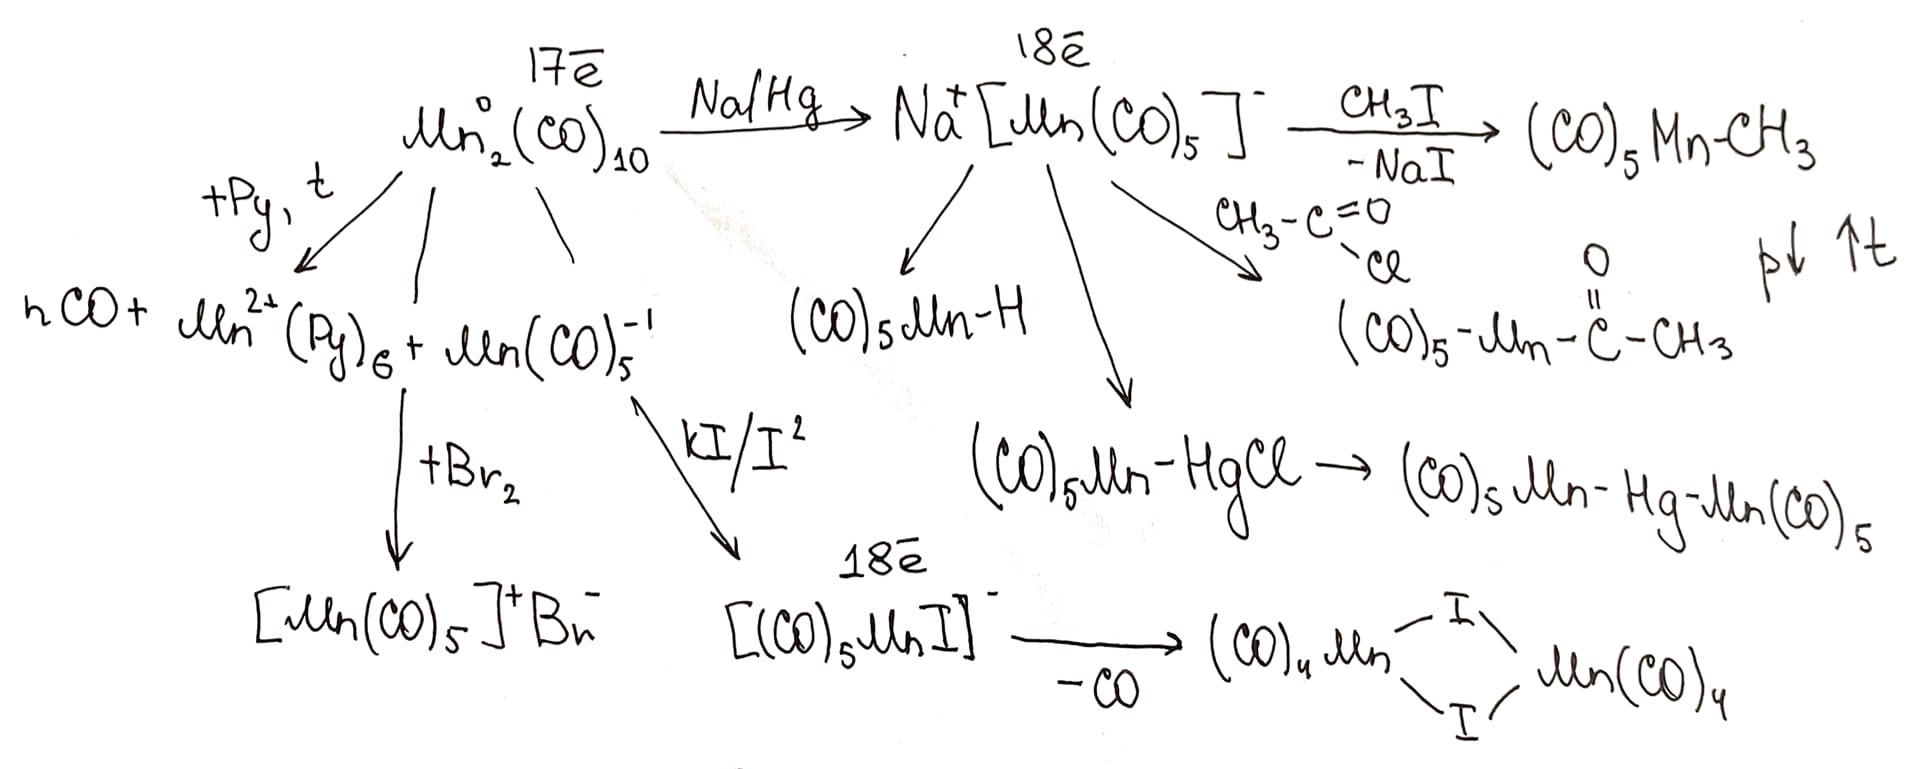
\includegraphics[scale=0.25]{zz1}}
\end{figure}
Свойства:
\begin{itemize}
	\item $Tc, Re$:
	\begin{itemize}
		\item $+ KOH \not = $
		\item $+ HCl \not = $
		\item $+ HNO_3\text{(к)} = HReO_4 + NO + H_2O$
		\item $+ H_2 \not = $
		\item $+ S  = ReS_2$
		\item $+ Cl_2 = ReCl_5$
		\item $+ F_2 = ReF_6$
		\item $+ O_2 =  Re_2O_7$		
	\end{itemize}
\end{itemize}
\textbf{Степень окисления $+1$} \\
$Mn^{+1}$ стабилизируется $\pi$-акцепторными $L$:
\[
Na_5\left[Mn^{+1}(CN)_6\right] \quad \left[Mn^{+1}(CO)_5\right]Br
\]
\textbf{Степень окисления $+2$} \\
$Mn^{+2}$ похож на $Mg^{+2}$, основный характер \\
Наиболее устойчивы оксо- и фторокомплексы 
$MnSO_4 + 6 H_2O = \left[Mn(H_2O)_6 \right]SO_4$ - октаэдр \\
$4KF + MnF_2 = K_4\left[MnF_6 \right]$ - октаэдр \\
$K_2\left[MnBr_4 \right]$ - тетраэдр \\
$\left[Mn(H_2O)_6 \right]^{2+} \quad \left[MnF_6 \right]^{4-} $
\begin{figure} [H]
	\centering {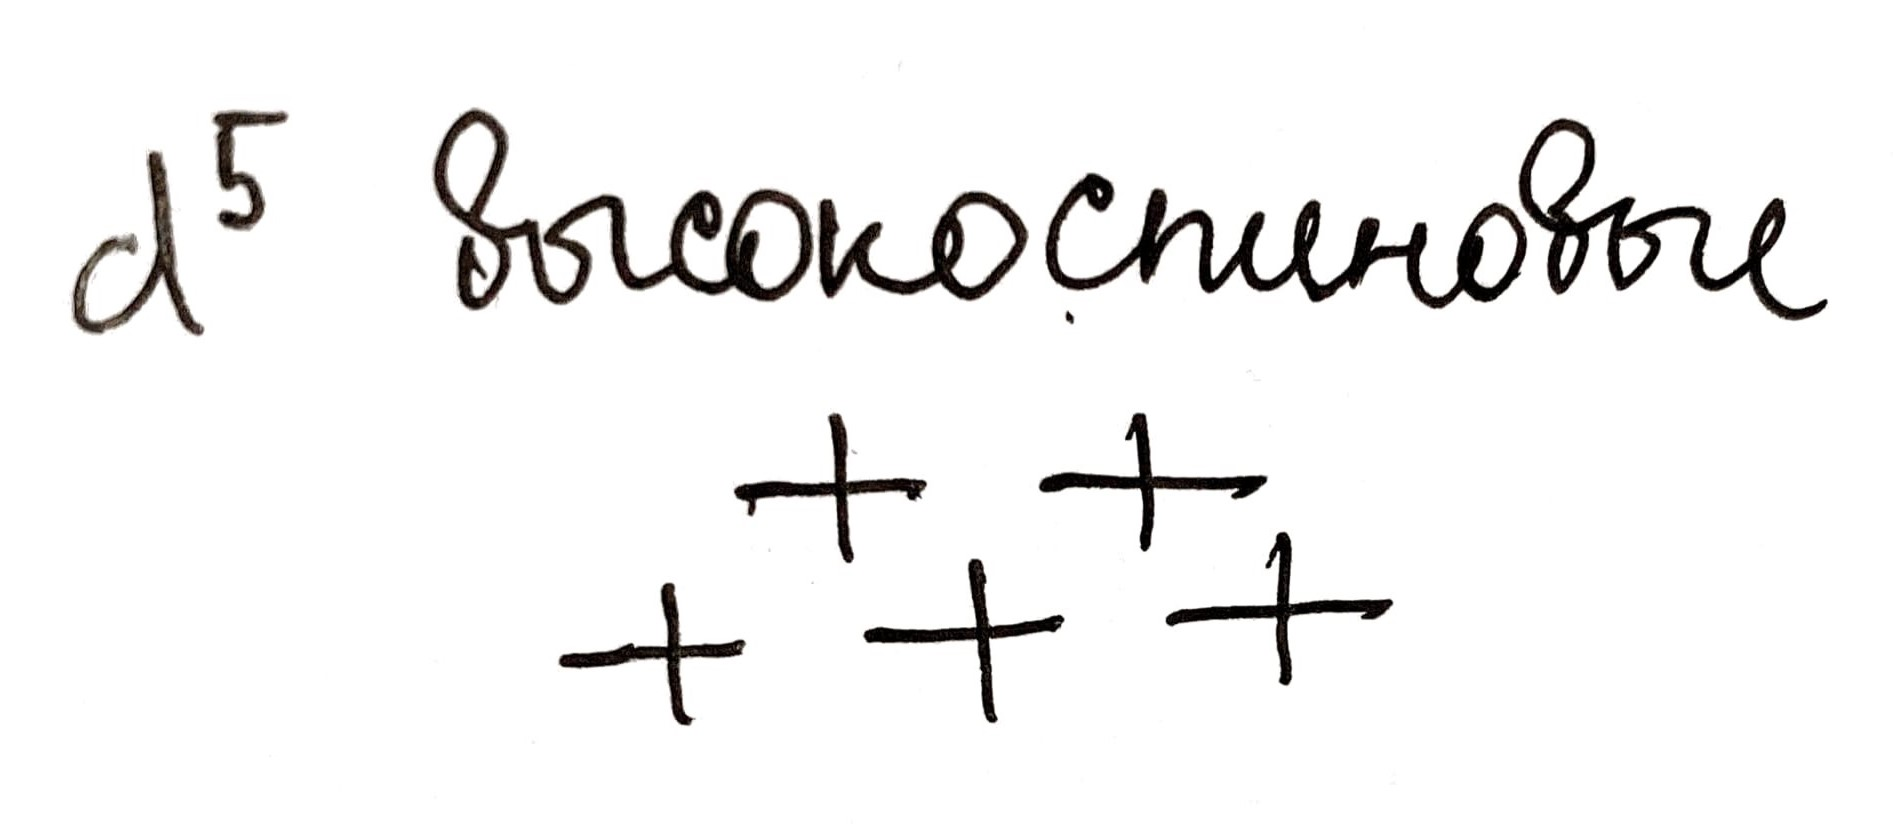
\includegraphics[scale=0.1]{zz3}}
\end{figure}
$ \left[Mn(CN)_6 \right]^{4-} $
\begin{figure} [H]
	\centering {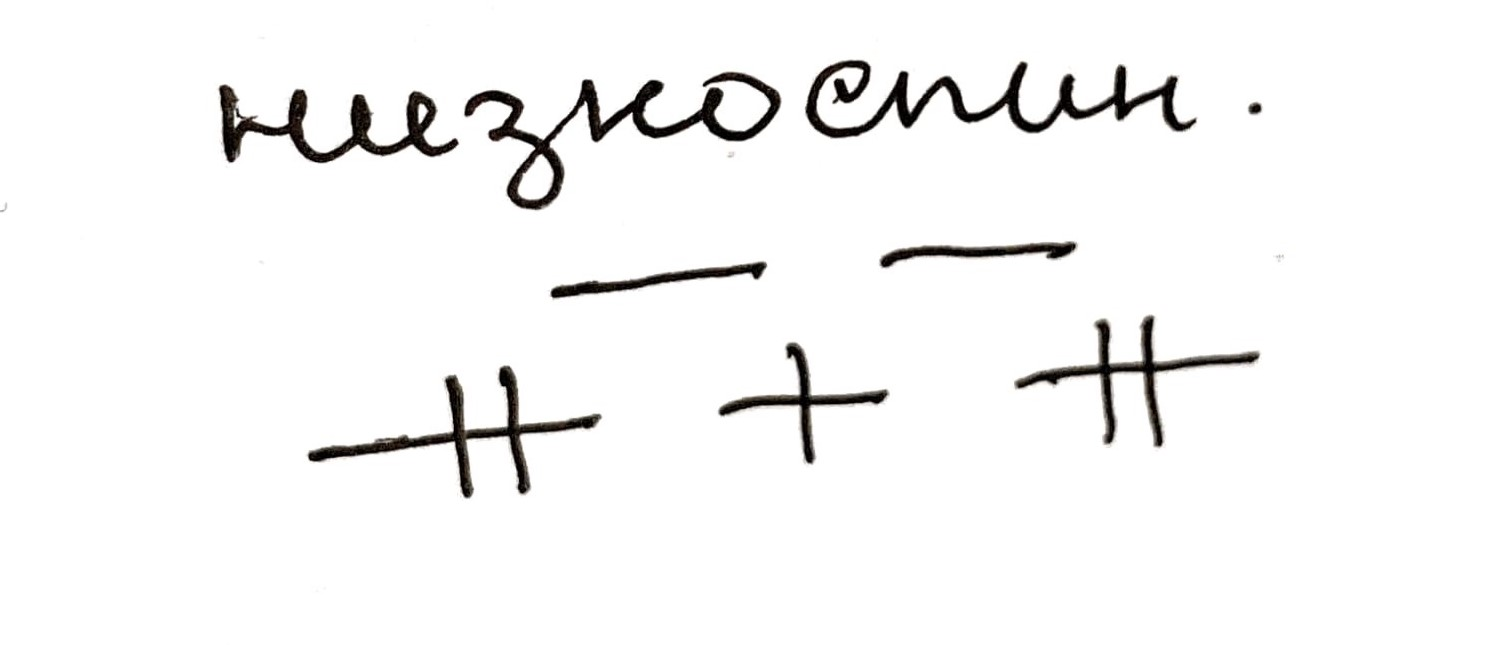
\includegraphics[scale=0.1]{zz2}}
\end{figure}
В низших степенях окисления $Re$ образует кластеры \\
\textbf{Степень окисления $+3$} \\
$\left[Mn(H_2O)_6 \right]^{2+}$ не стабилен, диспропорционирует \\
$Mn^{+3}$ можно стабилизировать $F^-, PO_4^{3-}, C_2O_4^{2-}$ \\
$\left[Mn(C_2O_4)_3 \right]$ - устойчивый хелатный комплекс \\
$\left[MnF_6 \right]^{3-}$ - октаэдрический, эффект Яна-Теллера: 
\begin{figure} [H]
	\centering {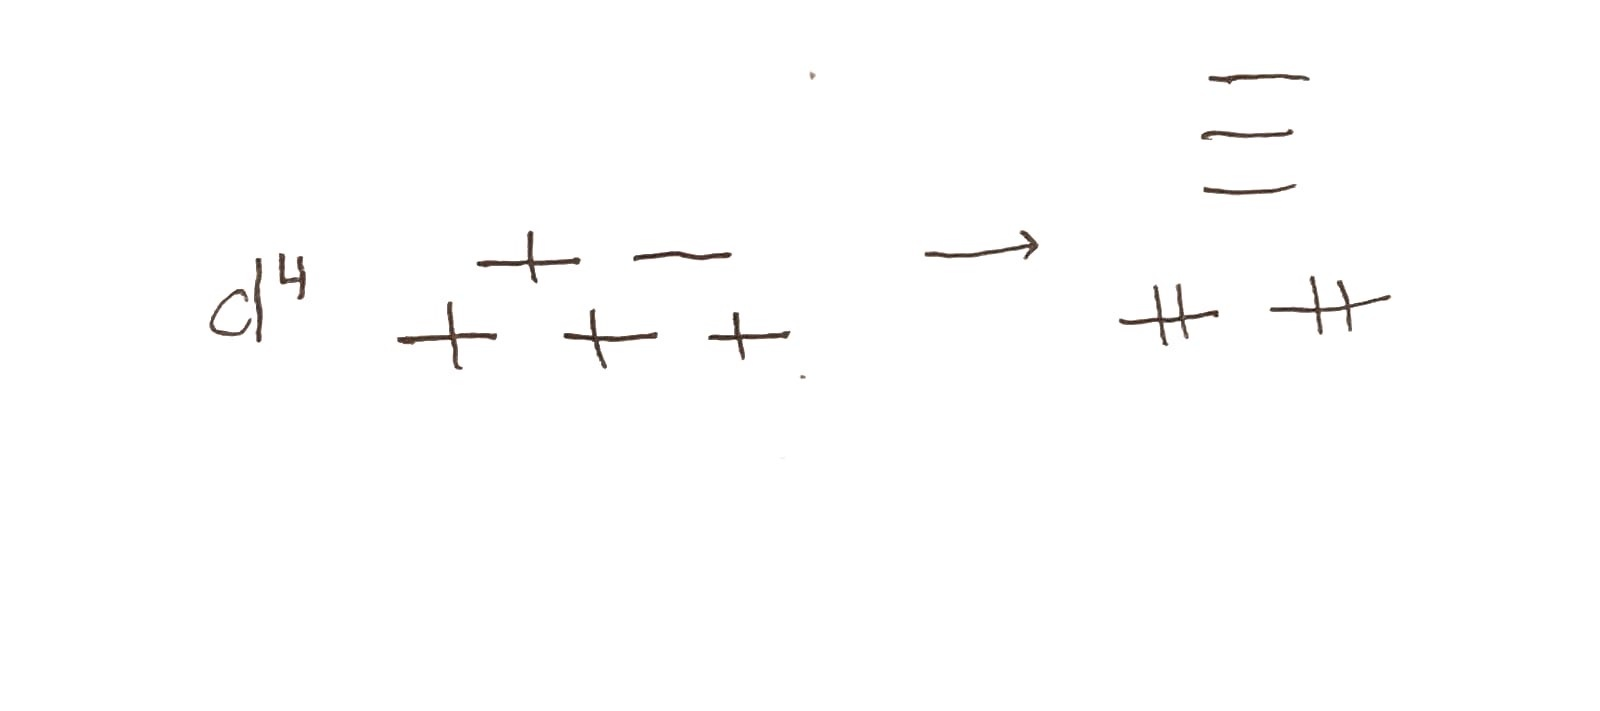
\includegraphics[scale=0.15]{zz4}}
\end{figure} 
Анионы $MnF_5^{2-}$ и $MnF_4^{-}$ имеют октаэдрическую структуру с искажением Я-Т. \\
$ReCl_3, ReCl_4$ - тримеры \\
$\left[MnCl_5 \right]^{2-} $ - квадратная пирамида. \\
Стабилизация $Mn(III)$:
\begin{align*}
KMnO_4 + 6 KF + 8HCl &= K_3\left[MnF_6 \right] + 4H_2O + 4KCl \\
KMnO_4 + H_2SO_4 + H_2O_2 &= K\left[Mn(SO_4)_2 \right] + 2O_2 + 4H_2O \\
KMnO_4 + 8Hcl + 2 KCl &= K_3\left[MnCl_6 \right] + 2Cl_2 + 4H_2O
\end{align*}
Хелатные более устойчивы:
\[
3MnO(OH) + 3H_2C_2O_4 + 3K_2C_2O_4 = 2K_3\left[Mn(C_2O_4)_3 \right] + 4H_2O
\]
Низкоспиновые:
\begin{align*}
2K_4\left[Mn^{+4}(CN)_6 \right] + H_2O_2 &= 2K_3\left[Mn^{+3}(CN)_6 \right] + 2KOH \\
K_3\left[MnF_6 \right] + 6KCN &= K_3\left[Mn(CN)_6 \right]	+ 6KF
\end{align*}
\textbf{Степень окисления $+4$} \\
$MnF_4$ - тетрамеры \\
$Mn^{+4}$ легко гидролизуется \\
Комплексы $Mn^{+4}$ (самые устойчивые - фторидные):
$\left[Mn(CN)_6 \right]^{2-}$ \\
\begin{align*}
MnF_2 + F_2 + KF &= K_2\left[MnF_6 \right] \\
K_2\left[MnF_6 \right] + SbF_3 &= K\left[SbF_6 \right] + MnF_2 + KF
\end{align*}
$TcO_2, ReO_2$ не растворяются в $H_2O$, в щелочах и в кислотах. \\
\textbf{Степень окисления $+5, +6$} \\
$\left[MnO_4 \right]^{2-}, \left[MnO_4 \right]^{3-}$ - существуют в щелочи, неустойчивы, диспропорционируют \\
Гидридные комплексы: $ TcH_9^{2-}, ReH_9^{2-} $
\begin{figure} [H]
	\centering {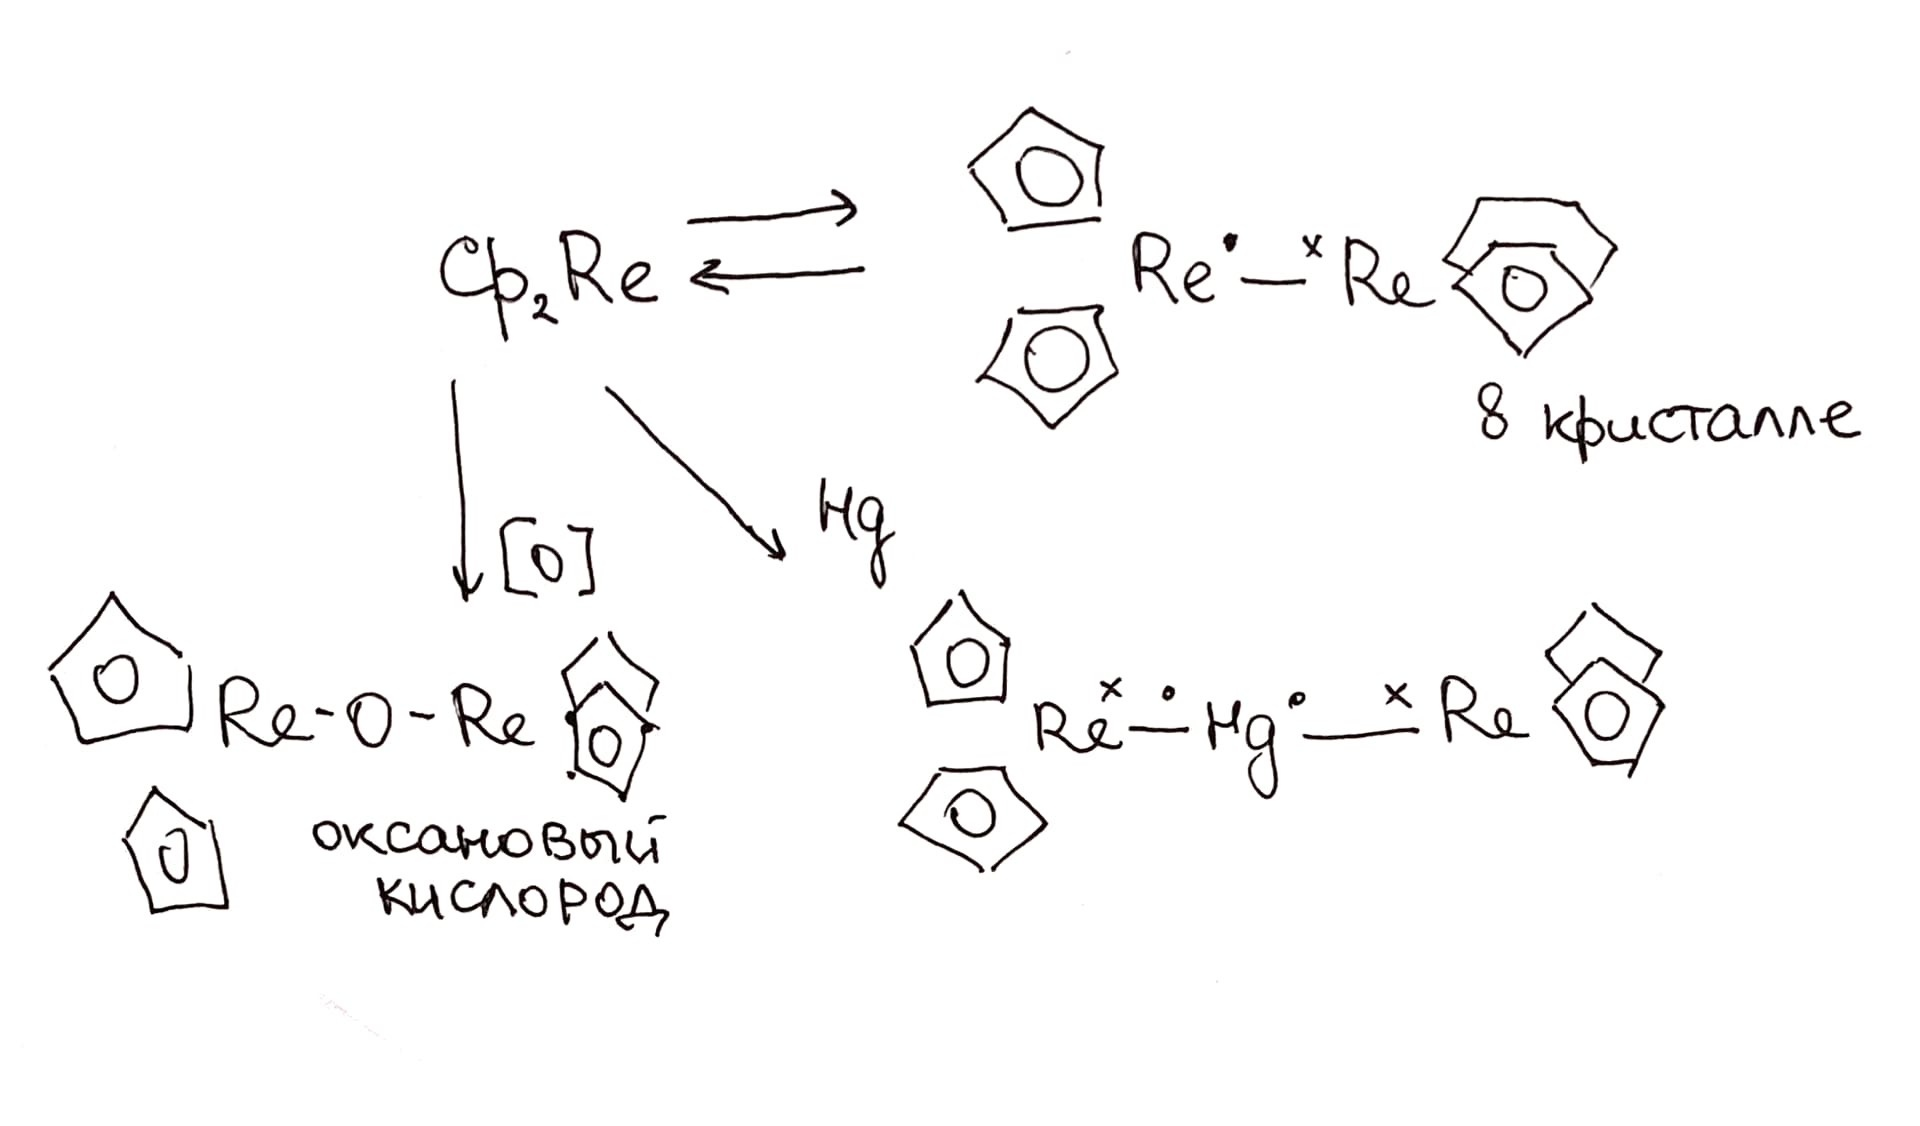
\includegraphics[scale=0.17]{zz5}}
\end{figure}

\section*{1.24 Соединения $Fe$, $Co$, $Ni$. Геометрия молекул в зависимости от природы лигандов, их электронное строение, способы получения и химическое поведение.}
\begin{itemize}
	\item $Fe$: $+1, +2, +3, (+4), (+5), +6$	
	\item $Co$: $+1, +2, +3, (+4)$
	\item $Ni$: $+1, +2, (+3), (+4)$
\end{itemize}
В природе (+ получение:)
\begin{itemize}
	\item $Fe_2O_3$ - гематит, $FeCO_3$ - железный шпат, $Fe_3O_4$ - магнетит.
	\begin{align*}
	Fe_2O_3 + CO &= Fe + CO_2 \\
	Fe_3O_4 + CH_4 &= 3 Fe + CO_2 + 2 H_2O	
	\end{align*}
	\item $CoAs_2$, $CoAs_3$.
	\begin{align*}
	3 CoS + 5O_2 &= Co_3O_4 + 3SO_2 \text{ (обжиг сульфида)} \\
	Co_3O_4 + 4 C &= 3 Co + 4 CO \text{ (восстановление)}
	\end{align*}	
	\item $NiS$ - колчедан.
	\begin{align*}
	2 NiS + 3O_2 &= 2NiO + 2SO_2 \\
	NiO +  C &= Ni + CO 
	\end{align*}
\end{itemize}
Свойства:
\begin{itemize}
	\item $Fe$:
	\begin{itemize}
		\item $+ O_2 = Fe_2O_3$
		\item $+ Hal = FeBr_3, FeI_2$
		\item $+ S = FeS_2$
		\item $+ P = FeP_4$
		\item $+ C = Fe_3C$
		\item $+ KOH \not =$
		\item $+ HCl = FeCl_2 + H_2$
		\item $+ HNO_3(\text{к}), H_2SO_4 (\text{к}) = \text{пассивация}$		
	\end{itemize}
	\item $Co$:
	\begin{itemize}
		\item $+ O_2 = Co_3O_4$
		\item $+ Hal = CoF_3, CoCl_2$
		\item $+ P = CoP_3$
		\item $+ HCl = CoCl_2 + H_2$
		\item $+ HNO_3(\text{к}), H_2SO_4 (\text{к}) = \text{пассивация}$
		\item $+ KOH \not =$
	\end{itemize}	
	\item $Ni$:
	\begin{itemize}
		\item + $O_2 = NiO$
		\item + $Hal = NiHal_2$
		\item + $HCl = NiCl_2 + H_2$
		\item + $HNO_3(\text{к}), H_2SO_4 (\text{к}) = \text{пассивация}$
		\item + $KOH \not =$
	\end{itemize}
\end{itemize}
\begin{figure} [H]
	\centering {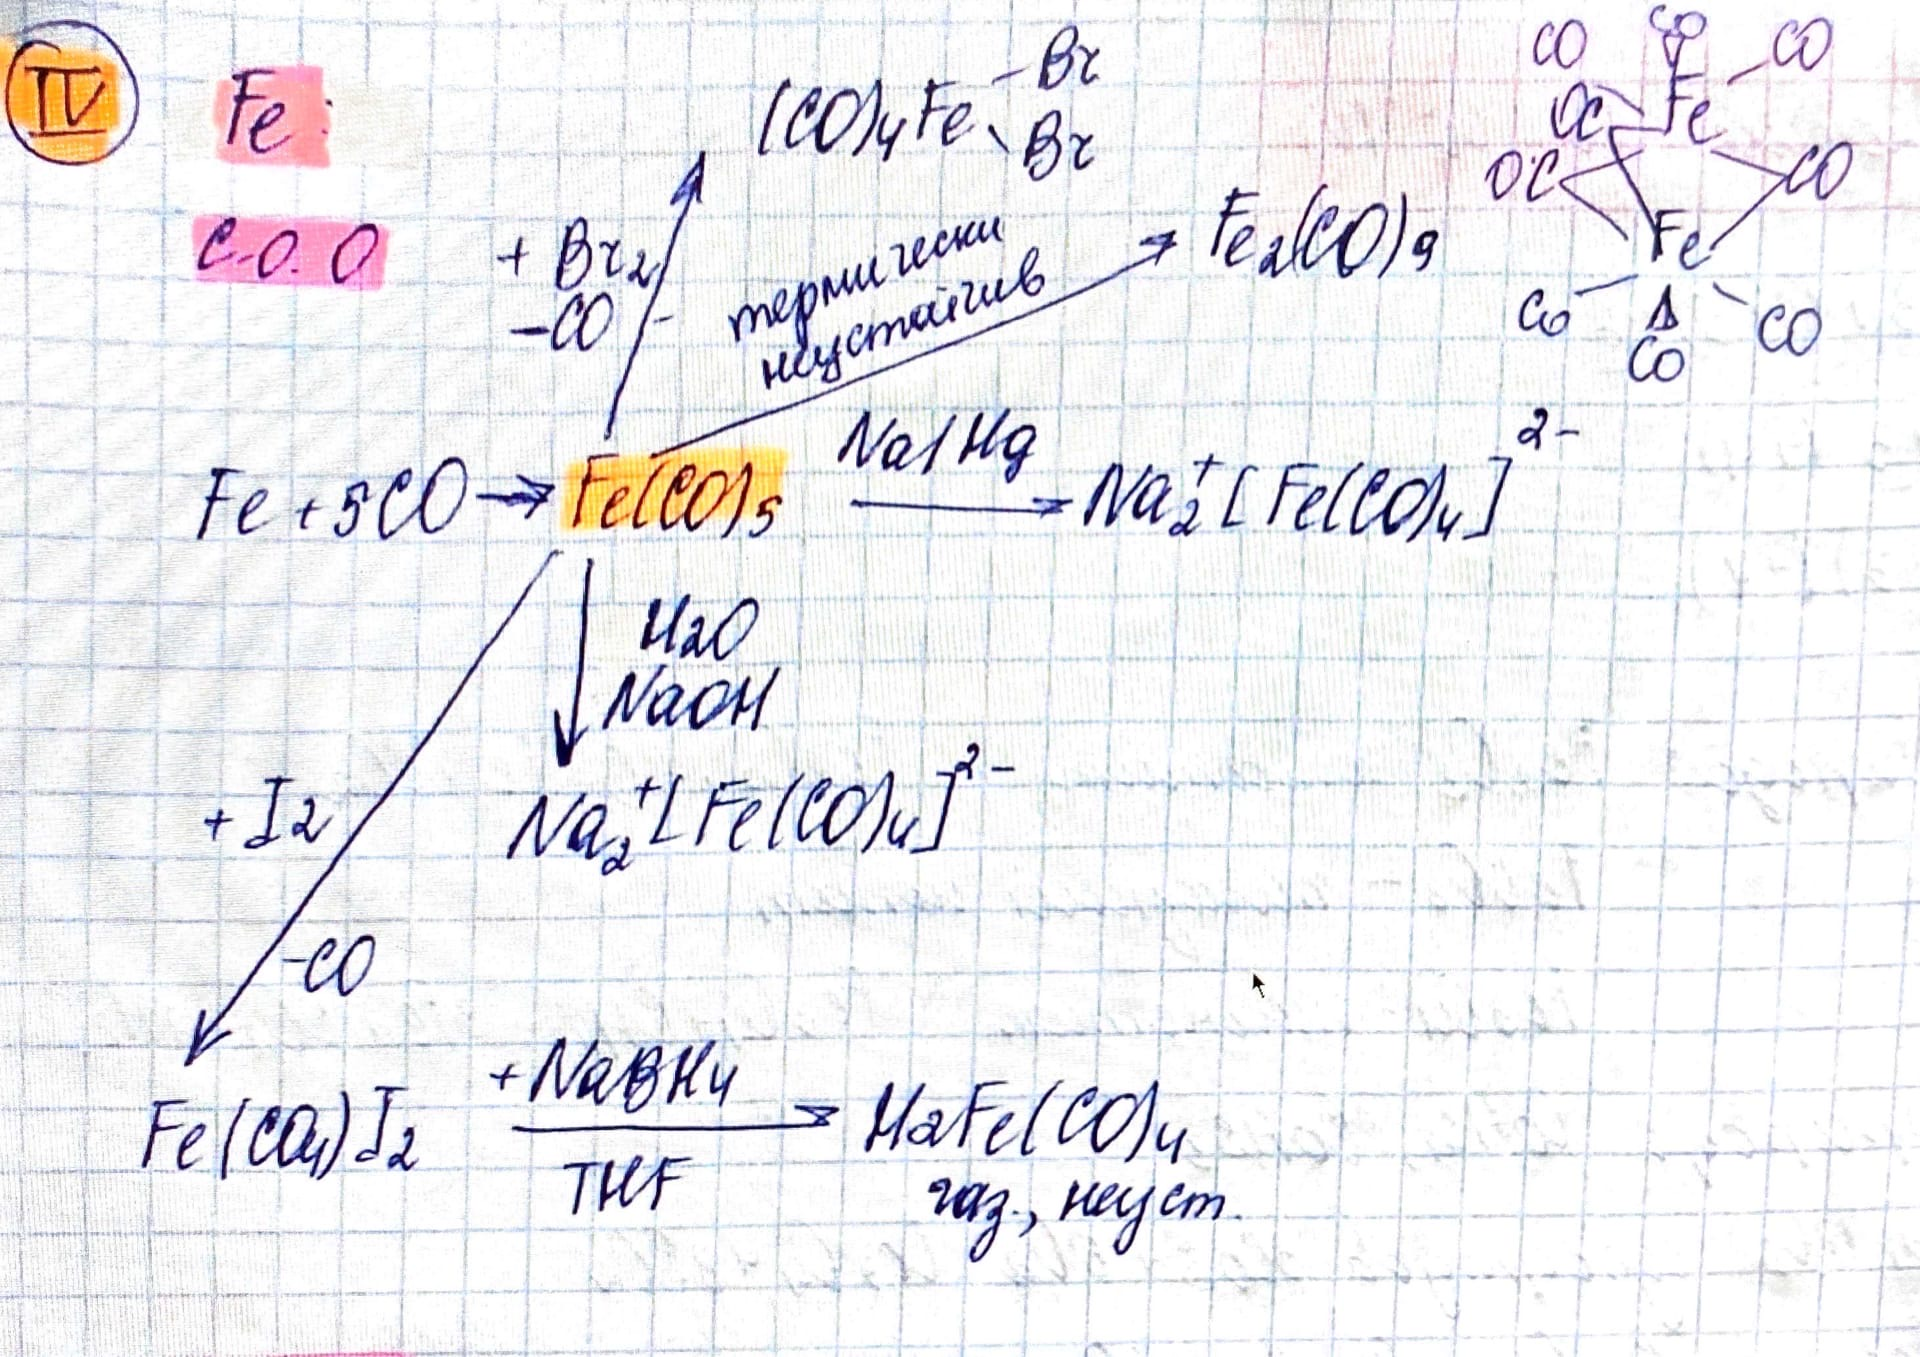
\includegraphics[scale=0.25]{ww1}}
\end{figure}
\textbf{Степень окисления $+2$}, ($d^6$)\\
\ul{Координационное число $6$}, высокоспиновые комплексы
\begin{align*}
&\left[Fe(H_2O)_6 \right]^{2-} \text{устойчивы аквакомплексы} \\
&FeCl_2 + 6 NH_3 = \left[Fe(NH_3)_6 \right]Cl_2 \\
&FeSO_4 + (NH_4)_2SO_4 = (NH_4)_2\left[Fe(SO_4)_2 \right] \cdot 6 H_2O \text{ (соль Мора)}
\end{align*}
Низкоспиновые комплексы с лигандами сильного поля: 
\[
\left[Fe(CN)_6 \right]^{4-}, \left[Fe(bpy)_3 \right]^{2+}, \left[Fe(phen)_3 \right]^{2+}, \left[Fe(en)_3 \right]^{2+}
\]
\ul{Координационное число $4$} \\
Тетраэдрические комплексы неустойчивы: $ \left[FeCl_4\right]^{2-}, \left[Fe(SCN)_4 \right]^{2-}$ \\
\ul{Координационное число $2$} \\
Объемные амидные лиганды: $\left[ Fe\{ N (SiMePh_2)_2 \}_2 \right]$ \\ \\
\textbf{Степень окисления $+3$}, ($d^5$)\\
Аммиакаты неустойчивы:
\[
FeBr_3 + 6NH_3 = \left[Fe(NH_3)_6\right]Br_3 = (H_2O) = \left[Fe(H_2O)_6\right]Br_3  
\]
Устойчивые с $\pi$-лигандами и хелатные:
\[
\text{высокоспиновые:} \left[Fe(H_2O)_6\right]^{3+}, \left[FeF_6\right]^{3-}, \left[Fe(ox)_3\right]^{3-}, \left[Fe(acac)_3\right] 
\]
\[
\text{низкоспиновые:} \left[Fe(CN)_6\right]^{3-}, \left[Fe(bpy)_3\right]^{3+}
\]
\ul{Координационное число $7$} \\
\[
\left[Fe(edba)(H_2O)\right]^{-}
\]
\ul{Координационное число $2$} \\
\[
\left[Fe(N(TMS)_2)_3\right] \text{ стабилизация амидными L}
\]
\textbf{Степень окисления $+4$} \\
$K_4FeO_4$ - тетраэдр, $d^4$, эффект Яна-Теллера \\
$12 KO_2 + Fe_3O_4 = 3K_4FeO_4 + 8 O_2$ - неустойчив в растворе, диспропорционирует \\
$FeF_2 + 2 CsF + XeF_2 = Cs_2\left[FeF_6 \right] + Xe$	\\ 
\textbf{Степень окисления $+5$} \\
$K_3FeO_4$ - тетраэдр \\
\textbf{Степень окисления $+6$} \\
Стабильность только в щелочном растворе:
\begin{align*}
2 Fe(OH)_3 + 10 KOH + 3 Br_2 &= 2K_2FeO_4 + 6KBr + 8H_2O \\
2K_2FeO_4 + 10H_2SO_4 &= 2Fe_2(SO_4)_3 + 3O_2 + 4K_2SO_4 + 10H_2O
\end{align*}
$FeO_4^{2-}$ - тетраэдр, парамагнитный \\ \\
$Co$: \\ \\
\textbf{Степень окисления $0$} \\
\[
2Co + 8CO = Co_2(CO)_8
\]
В двух формах:
\begin{figure} [H]
	\centering {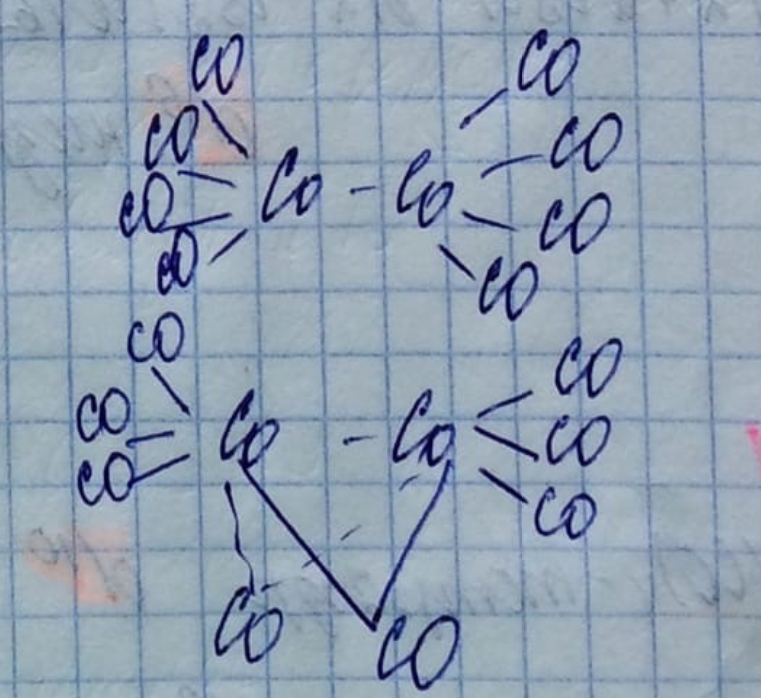
\includegraphics[scale=0.7]{ww2}}
\end{figure}
Образование мостиковой структуры более выгодно из-за размера ионов и участия $d$-орбитали.
\[
Co + 4CO + \frac12 H =   \left[Co(CO)_4 H \right] \text{ - сильная кислота}
\]
$Co_4(CO)_{12}$ - тетраэдрический кластер \\
\textbf{Степень окисления $+1$} \\
$\left[Co(PMe_3)_4\right]^+$ - тетраэдр \\
\textbf{Степень окисления $+2$}, ($d^7$)\\
нет предпочтительной конфигурации \\
\ul{Координационное число $2$} \\
Линейное строение $\left[ Co\{ N (SiMe_3) \}_2 \right]$ \\
\ul{Координационное число $3$} \\
Треугольное: $\left[ Co\{ N (SiMe_3) \}_2 (pph_3)\right], \left[ Co\{ N (SiMe_3)_2 \}_3 \right] $    \\
\ul{Координационное число $4$} \\
Тетраэдр: $\left[Co(Cl)_4 \right]^{2-}, \left[Co(OH)_4 \right]^{2-}  $ \\ 
\ul{Координационное число $5$} \\
Пирамида: $\left[Co(CN)_5 \right]^{3-}$   \\
\ul{Координационное число $6$} \\
Октаэдр: $\left[Co(H_2O)_6 \right]^{2+}$    \\
\ul{Координационное число $7,8$} \\
С краун-эфирами \\
\textbf{Степень окисления $+3$}, ($d^6$)\\
Устойчивы низкоспиновые комплексы $Co$ с $L$ сильного поля (кроме $\left[CoF_6 \right]^{3-}$) \\
Аквакомплекс $\left[Co(H_2O)_6 \right]^{3+}$ \\ \\
Аммиакаты с различным составом, инертны:
\[
\left[Co(NH_3)_6 \right]Cl_3, \quad \left[CoCl_2(NH_3)_4 \right]Cl, \quad \left[CoCl_3(NH_3)_3 \right]
\]
\textbf{Степень окисления $+4$}, ($d^5$)\\ 
Низкоспиновый:
\[
CoCl_2 + 2CsCl + 3 F_2 = Cs_2\left[CoF_6 \right] + 2Cl_2
\] \\ 
$Ni$: \\ \\
\textbf{Степень окисления $0$}, ($d^10$)\\
$Ni(CO)_4$ - тетраэдр \\
\textbf{Степень окисления $+1$}\\
Цианиды:
\[
K_2\left[Ni^{+2}(CN)_4 \right] = Na/Hg = K_4\left[Ni^{+1}(CN)_6 \right] = K/NH_3\text{(ж)} = K_4\left[Ni^{0}(CN)_4 \right]
\]
\textbf{Степень окисления $+2$}\\
\ul{Координационное число $4$} \\
$NiBr_2 + 2KBr = K_2\left[NiBr_4 \right]$ - устойчив, тетраэдр \\
Тетраэдры только с $L$ слабого поля \\
Квадратные с $L$ сильного поля: \\
$NiCl_2 + 4 KCN = 2 KCl + K_2\left[Ni(CN)_4 \right]$ \\
\ul{Координационное число $6$} \\
$\left[Ni(H_2O)_6 \right]^{2+}, \quad \left[Ni(NH_3)_6 \right]^{2+}, \quad \left[Ni(bpy)_3 \right]^{2+}$, олигомер $\left[Ni(acac)_2 \right]$ \\
\textbf{Степень окисления $+3$}, ($d^7$)\\
Относительно устойчивы фторокомплексы, сильные окислители, стабилизация $\sigma$ $\pi$-донорными $L$. \\
$ \left[NiBr_3(PEt_3)_2 \right] $ - низкоспиновый \\
$ \left[Ni_3(CH_3COO)_6 \right]^{3-} $ \\
\textbf{Степень окисления $+4$}, ($d^5$)\\
Стабилизация в гетерополисоединениях $(NH_4)\left[NiMo_9O_{32}\right]$ \\
$\left[NiF_6\right]^{2-}, \quad \left[NiIO_6\right]$ - окислители

\section*{1.25 Соединения $Ni$, $Pd$, $Pt$. Геометрия молекул в зависимости от природы лигандов, их электронное строение, способы получения и химическое поведение.}
\section{Вопрос 1}
\subsection{ Соединения Ni, Pd, Pt. Геометрия молекул в зависимости от природы лигандов, их электронное строение, способы получения и химическое поведение.}

\textbf{Степени окисления}\\
$Ni$-- 0, +1, \textbf{+2}, +3 , +4\\
$Pd$-- 0, \textbf{+2}, +3, +4\\
$Pt$-- 0, \textbf{+2},\textbf{+4}, +5, +6

Сверху вниз повышается устойчивость карбонильных комплексов

\textbf{КЧ:}\\
3: $[Pt(Ph_3)_3]$\\
4:  $[Pt(Cl_4)]^{2-}$ - плоский квадрат $\Rightarrow d^8$\\
$[NiCl_4]^{2-}$ - тетраэдр $\Rightarrow d^8$

6: для $Ni[Ni(H_2O)_6]^{2+}$ и $Pd(IV), Pt(IV), [PtF_6]^{2-}$

\textbf{Получение}

Pd - отходы производства от Ni, Cu\\
Pt - саморододная в земной коре

\textbf{Химические свойства}\\
$$Pd/Pt + F_2 \rightarrow PdF_4 / PtF_6$$
$$Pd + O_2 \rightarrow PdO$$
$$Pt + HNO_3 + HCl \rightarrow H_2[PtCl_6]_6 + NO + H_2O$$
$$Pd + HNO_3 + HCl \rightarrow Pd(NO_3)_3 + NO_2 + H_2O$$

$$PtO_2\cdot 2H_2O + 2NaOh \rightarrow Na_2[Pt(OH)_6]$$
$$PtO_2\cdot 2H_2O  + HCl \rightarrow H_2[PtCl_6] + 4H2O$$
$$H_2[PdCl_6] + 2NaI \rightarrow H_2[PdCl_4] + I_2 + 2NaCl$$

\textbf{Галогениды}
$$PtCl_2 \xrightarrow{F_2, t} PtF_5$$
$$Pt \xrightarrow{F_2,t} PtF_5$$

$PdF_6$ и $PdF_5$ неизвестны, но:
$$PdF_6 + KrF_2 + O_2 \rightarrow  [O_2]^+[PdF_6]^{2-} + Kr$$

Высший галогенид $PdF_4$

$$O_2 + PtF_6 \rightarrow [O_2]^+[Pt^{+5}F_6]^-$$
$$2PtF_6 + 7CO \xrightarrow{HF, t} [Pt(CO)_4][PtF_6] + 3COF_2$$
$$PtF_6 + 6CO + SbF_5  \xrightarrow{p,t} [Pt(CO)_4][Sb_2F_{11}]_2 + 2COF_2$$

$$[Pt(CO)_4]^{2+}$$


$\textbf{Pd} : PdF_4$\\
$\textbf{Pt} : PtCl_4, PtBr_4, PtI_4$

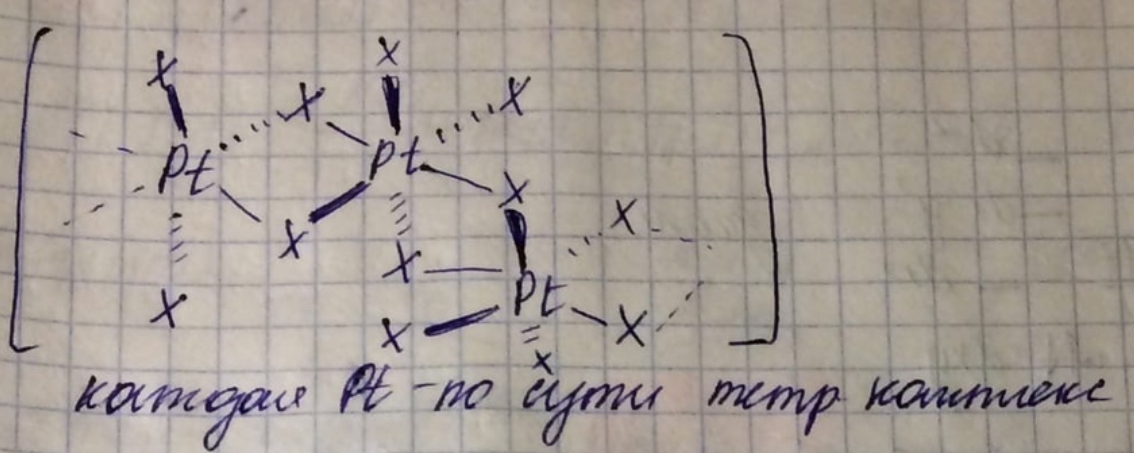
\includegraphics[scale=0.6]{25v1.png}

$$M \xrightarrow{KCl} K_2[MCl_6] (M = Pd, Pt)$$
$$K_2[PtCl_6] \xrightarrow{B_2F_3} K_2[PbF_6]$$
$$PtCl_4 \xrightarrow{HCl} H_2[PtCl_6]$$
$$PtCl_4 \xrightarrow{KCl} H_2[PtCl_6]$$
$$PtCl_4 \xrightarrow{KI} K_2[PtI_6]$$

$$trans-[PdCl_2(NH_3)_2] + Cl_2 \rightarrow trans-[PdCl_4(NH_3)_2]$$

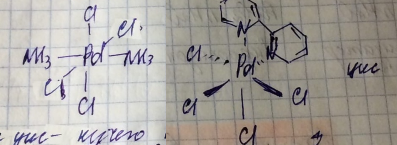
\includegraphics{25v2.png}

В цис- ничего не получится, если только N не сразу ориентированы

\textbf{Соединения Pd, Pt в с.о. +2}

$$M^{2+} + 2e \leftrightarrows M$$
$M = Ni, E^0 = -0,25 B$\\
$M = Pd, E^0 = 0,95 B$\\
$M = Pt, E^0 = 1,18 B$

$$[PtCl_6]^{2-} \xrightarrow{SO_2, HCl} H_2PtCl_4 \xrightarrow{NH_{3(konc)}} [Pt(NH_3)_4]Cl_2$$

$$[Pt(NH_3)_4]Cl_2 + [PtCl_4]^{2-} \rightarrow [Pt(NH_3)_4][PtCl_4] + 2Cl^-$$
$$[PtCl_4]^{2-} + 2NH_3\xrightarrow{aq.solution} cis-[PtCl_2(NH_3)_2] + 2Cl^-$$
$$[PtCl_4]^{2-} + 2HCl \xrightarrow{aq. solution} trans-[PtCl_2(NH_3)_2] + 2[NH_4]^+$$

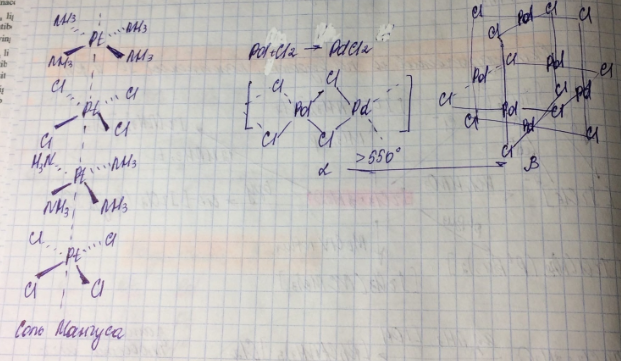
\includegraphics{25v3.png}
\\

\textbf{Транс-влияние и транс-эффект}

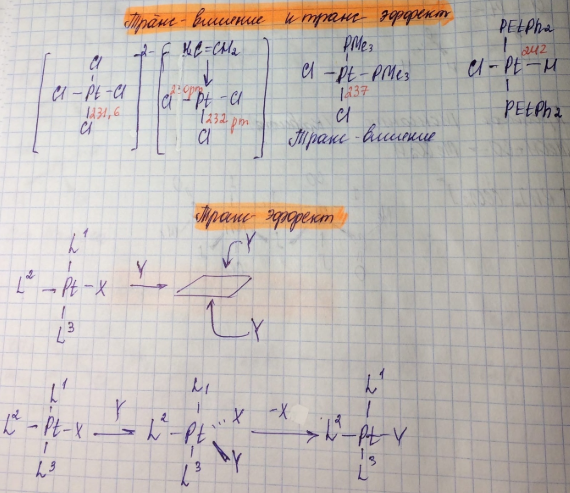
\includegraphics{25v4.png}\\
\\

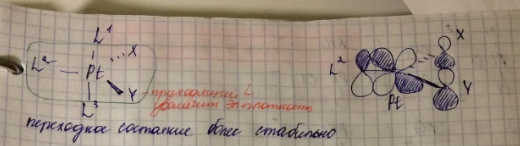
\includegraphics{25v5.png}

В основном состоянии:\\
Транс-влияние -- степень, в которой лиганды ослабляют связь в транс-положении в основном состоянии комплекса (коррелирует с $\sigma$-донорными связями, в связывании участвуют одни и те же орбитали M)

В переходном состоянии:\\
Транс-влияние коррелирует с $pi$-акцепторной способностью лиганда, "приходящий" лиганд увеличивает электронную плоскость на атоме М, акцепторный лиганд в транс-положении стабилизирует переходное состояние.

Транс-эффект можно считать комбинацией обоих эффектов

Транс $\sigma$-донор : $OH^- < NH_3 < Cl^- < Br^- < CN^- < CH_3^- <I^- < SCN^- < PR_3 , H^-$\\
Транс $\pi$-акцептор $Br^- < I^- < NCS^- < NO_2^- < CN^- < CO , C_2H_4$

$$[Pt(NH_3)_4]^{2+} + Cl^- \rightarrow [PtCl(NH_3)_2]^- \rightarrow trans-[PtCl_2(NH_3)_2]$$

$$[PtCl_4]^{2-} + NH_3 \rightarrow [PtCl_3(NH_3)]^- \rightarrow cis-[PtCl_2(NH_3)_2]$$

\textbf{Никель}

$Ni(CO)_4$ - тетраэдр, $d^{10}$\\
Цианиды: $K_2[Ni(CN)_4] \xrightarrow{Na/Hg} K_4[Ni_2(CN)_6] \xrightarrow{K/NH_{3(liq)}} K_4[Ni(CN)_4]$

С.О +2, к.ч. =4\\
$$NiBr_2 + 2KBr \rightarrow K_2[NiBr_4]$$
Устойчивый тетраэдр

Тетраэдры - только с лигандами слабого поля\\
Квадраты - с лигандами сильного поля, диамагнитны.

$$NiCl_2 + 4KCN \rightarrow 2KCl + K_2[Ni(CN)_4]$$

к.ч.=6 $[Ni(H_2O)_6]^{2+}, [Ni(NH_3)_6]^{2+}, [Ni(bipy)_3]^{2+}$\\
Антогомер $[Ni(acac)_2]$

С.О. +3\\
$d^7$ относительно устойчивы фторокомплексы, сильные окислители\\
Стабилизация $\sigma,\pi$-донорными лигандами\\
$[NiBr_3(PEt_3)_2]$ - низкоспиновый\\
$[Ni_3(CH_3COO)_6]^{3-}$

Коорд. соединение $M_3[Ni(CH-NO)_6]$

С.О.  +4

$d^5$\\
Стабилизация в гетерополисоединениях $(NH_4)_6[NiMo_9O_{32}]$\\
$[NiF_6]^{2-},  [NIO_6]$ - окислители

\textbf{Комплексы никеля}

$[NiCl_4]^{2-} [NiBr_4]^{2-}$  - тетраэдр\\
$[Ni(CN)_4]^{2-}$ - плоскоквадратный\\
$[Ni(CN)_5]^{3-}$ - тригональная бимирамида или кв.пирамида\\
$Fe(CO)_5$ - что лучше тригональная бипирамида или квадратная пирамида? Здесь - тригональная бипирамида

Зависит от природы катиона ( нарушает постулат:  признак ионных соединений -- полная независимость катиона и аниона)\\

$[NiF_6]^{4-}$ - октаэдр\\

$$NiBr_2 + PEtPh_2 \rightarrow [Br_2Ni(PEtPh_2)_2]$$

$$[Br_2Ni(PEtPh_2)_2] \leftrightarrows [Br_2Ni(PEtPh)_2]$$

$[Br_2Ni(PEtPh_2)_2]$ - зеленый, тетраэдр, парамагнитный, 2 неспаренных электрона\\

$[Br_2Ni(PEtPh)_2]$ - коричневый, плоскоквадратный, диамагнитный\\

Энергии близки их можно закристаллизовать

\textbf{Замена циклопентадиенильного кольца}

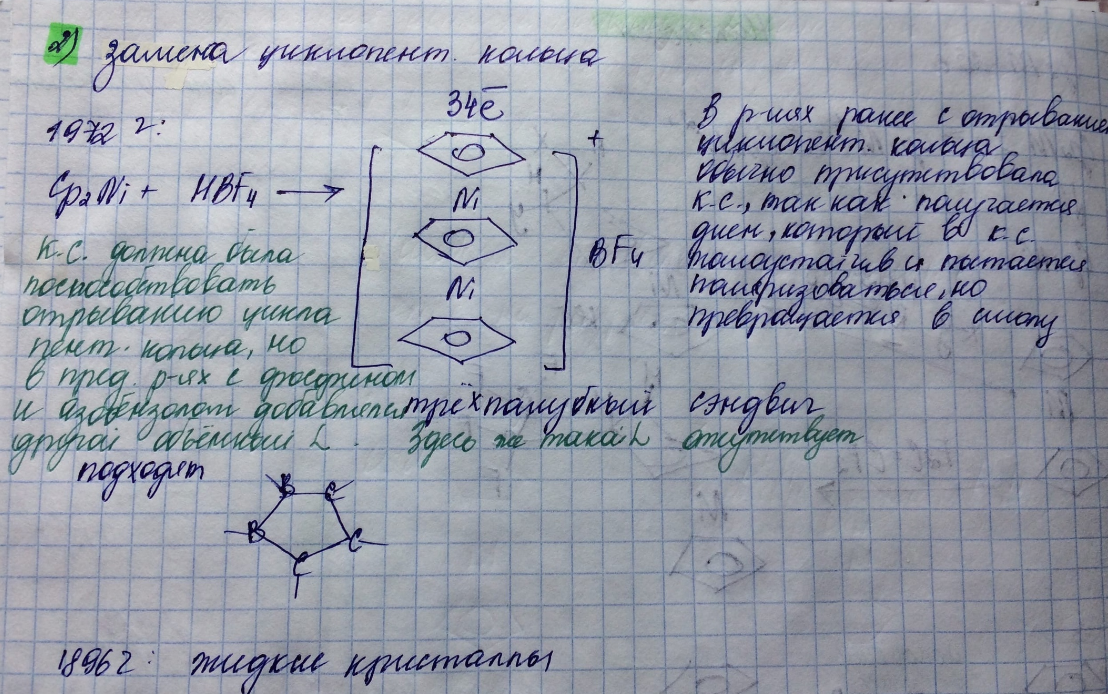
\includegraphics[scale=0.95]{25v6.png}

\textbf{Никелоцены}\\
\\

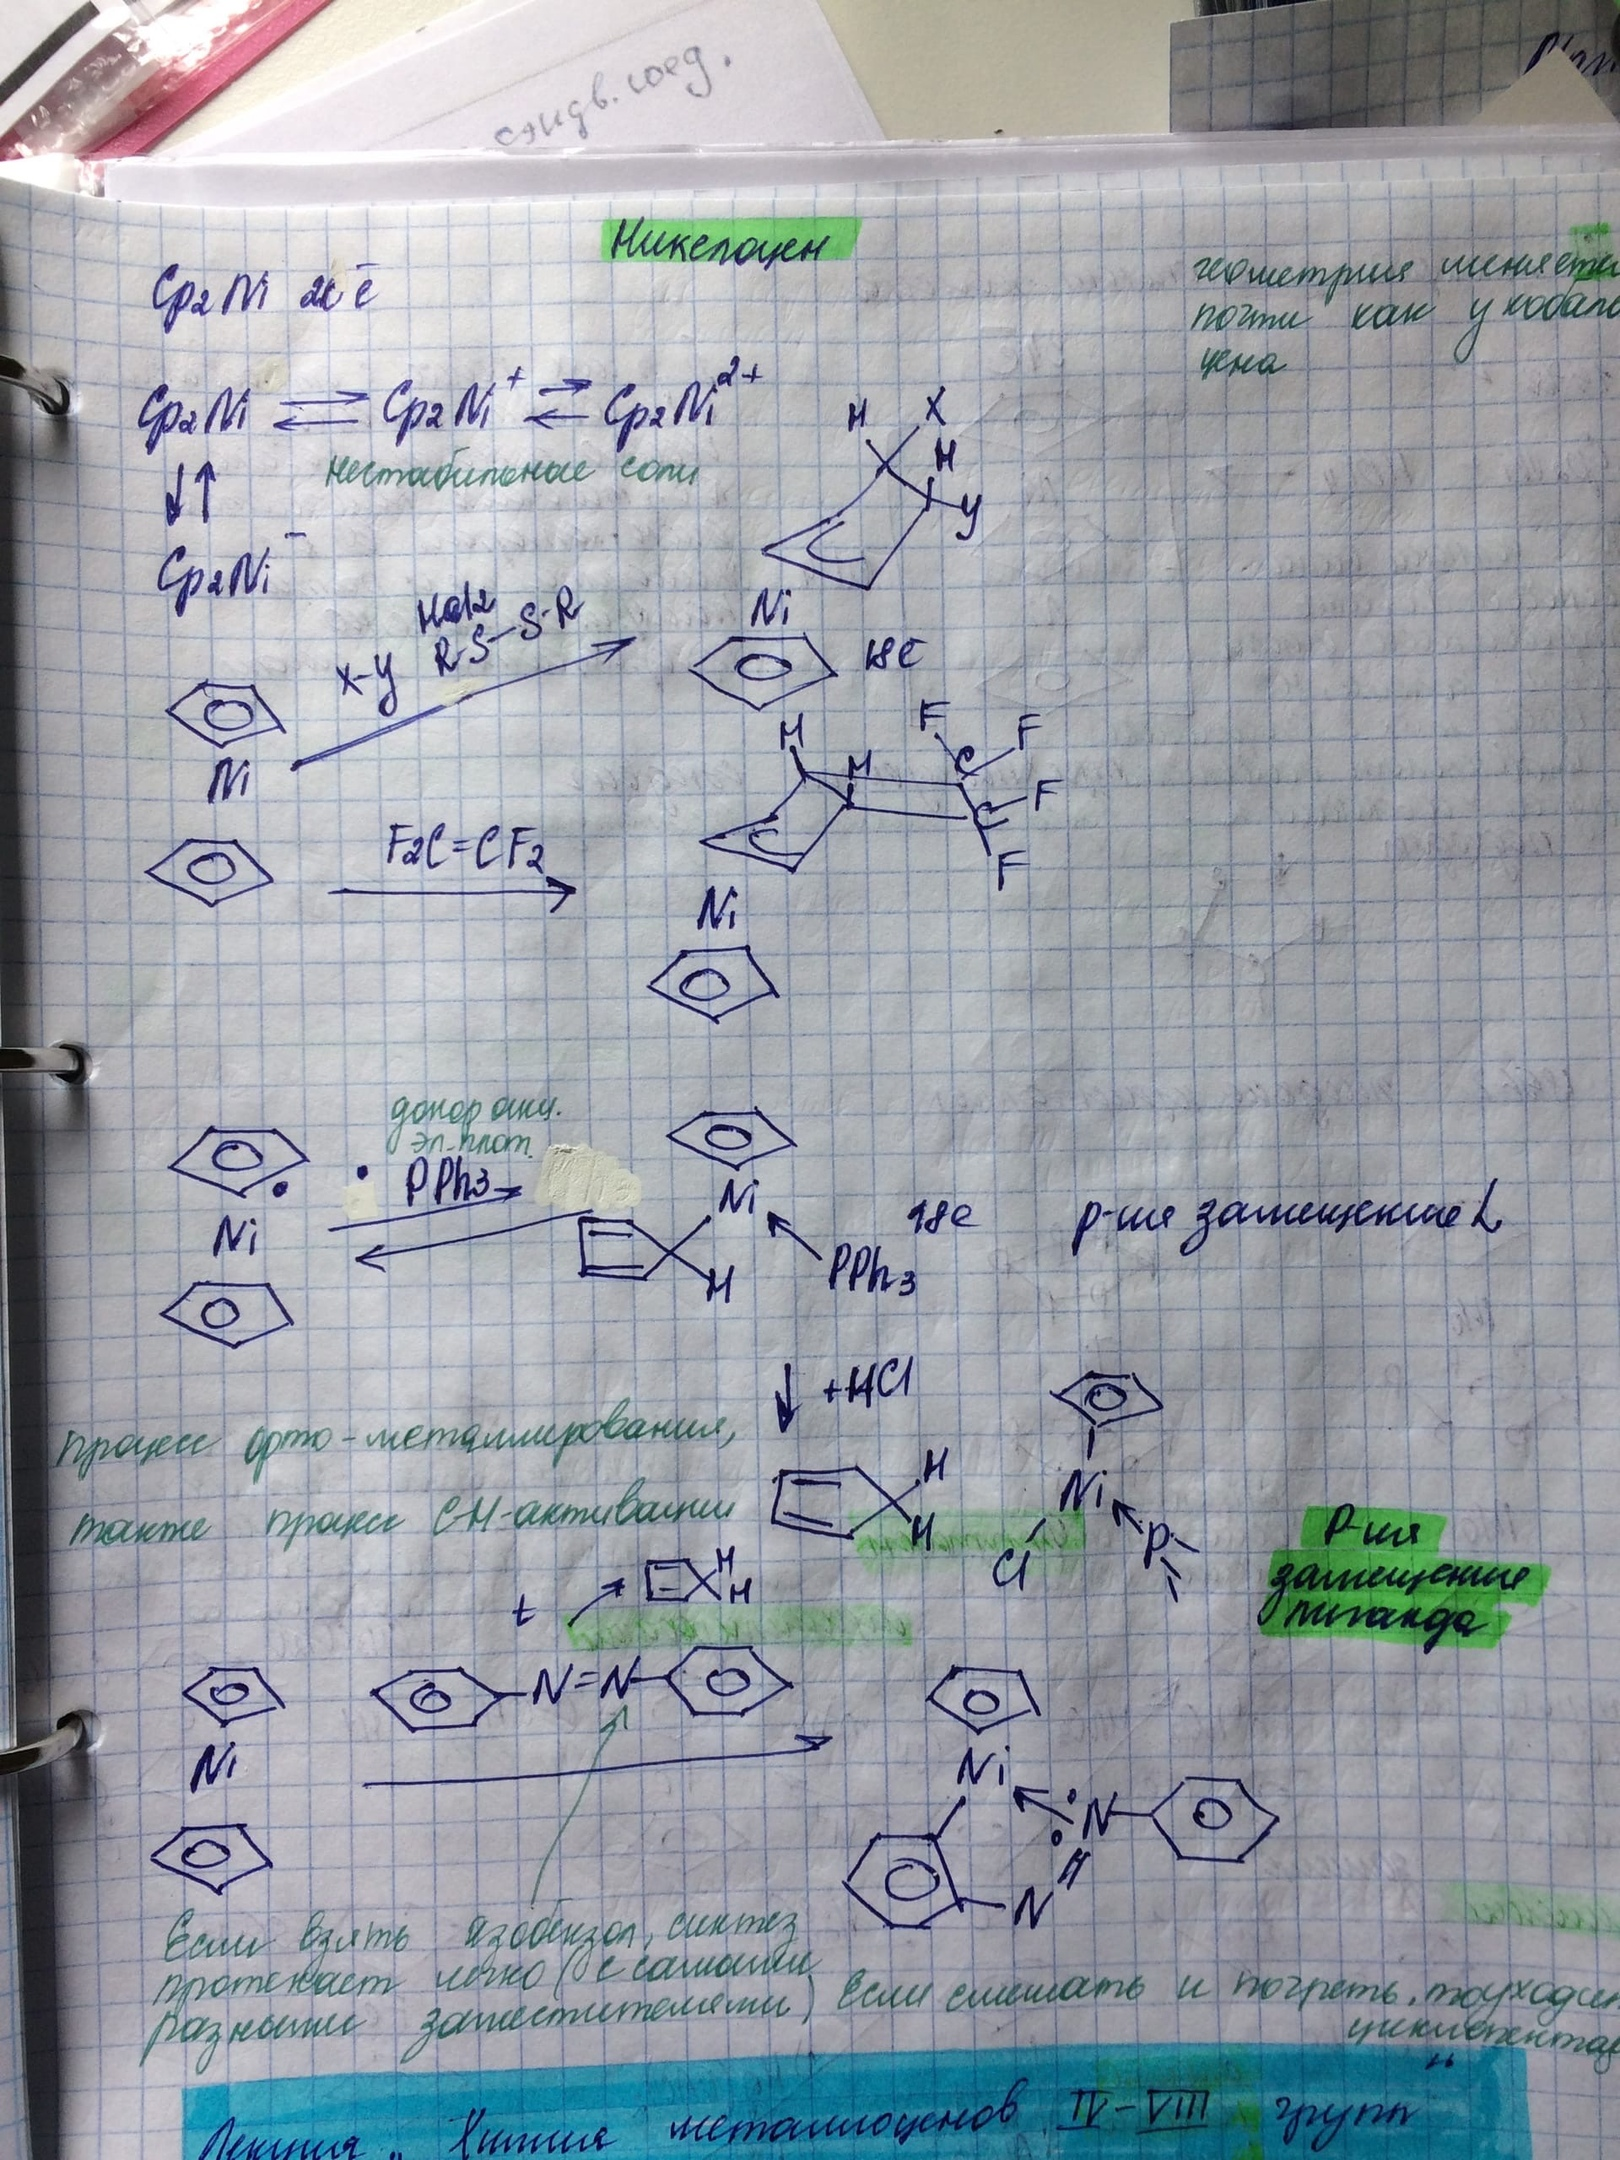
\includegraphics[scale=0.3]{25v7.png}

\section*{1.26 Соединения лантанидов. Геометрия молекул в зависимости от природы лигандов, их электронное строение, способы получения и химическое поведение.}

\section*{1.27 Сэндвичевые соединения переходных металлов с параллельными циклами (гомолигандные, гетеролигандные, многопалубные). Способы получения и условия стабильности, геометрия, электронное строение, свойства.}
\begin{figure} [H]
	\centering {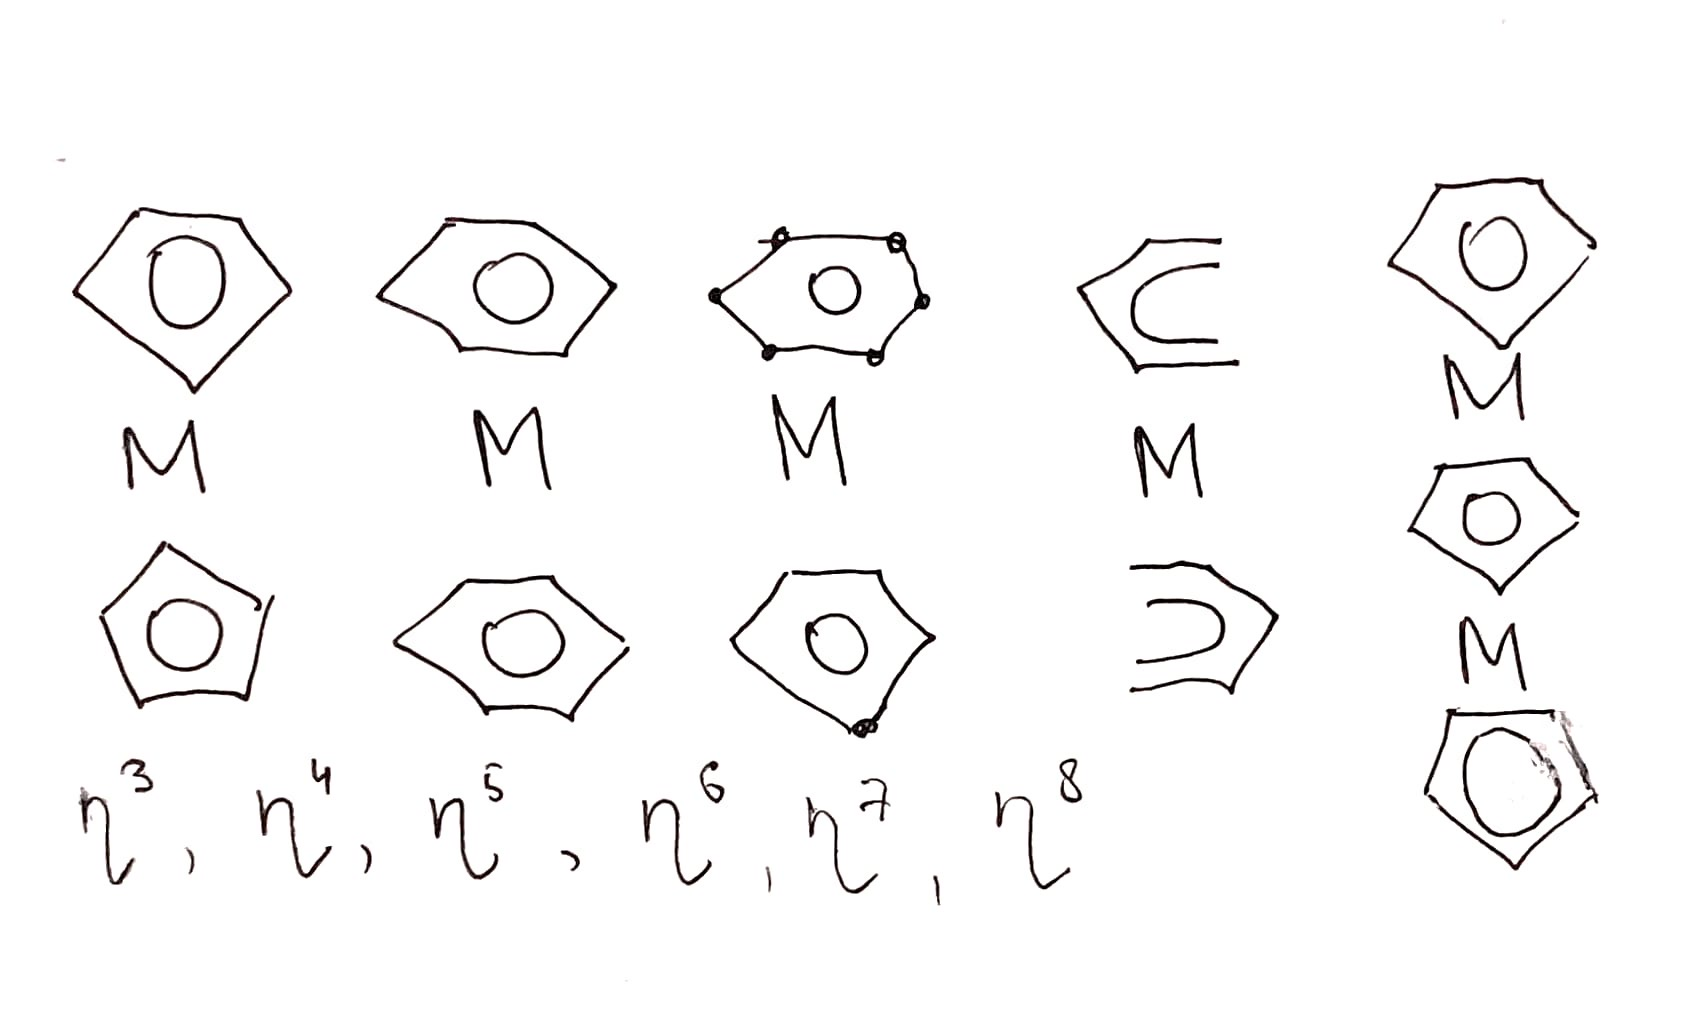
\includegraphics[scale=0.17]{xx1}}
\end{figure}
Самый устойчивый ферроцен $Cp_2Fe$ \\
Ароматичны \\
\textbf{Получение:}\\
\begin{itemize}
	\item Соль $Me$ + $Cp$-реагент
	\[
	MCl_2 + CpNa = Cp_2M \qquad (M = V, Cr, Mn, Fe, Co)
	\]
	\item Соль $Me$ + $CpH$ + осн.
	\[
	FeCl_2 + 2CpH + 2Et_2NH = Cp_2Fe + 2Et_2NH_2Cl
	\]
	\item Синтез Фишера-Хафнера
	\begin{align*}
	3CrCl_3 + 2Al + 6ArH = AlCl_3, H_2O &= \left[(ArH)_2 Cr \right]^{+} + Al^{3+} \\
	\left[(ArH)_2 Cr \right]^{+} + Na_2S_2O_4 + KOH &= (\eta^6 - ArH)_2Cr 
	\end{align*}
	\item Циклотримеризация алкинов
	\[
	(C_6H_5)_3Cr(THF)_3 + H_3C-C\equiv C-CH_3 = H_2O = (PhH)_2Cr
	\]
	\item Соконденсация из паров
	\[
	Ti\text{(г)} + 2PhH \text{(г)} = Ti(PhH)_2
	\]
	\item Получение трехпалубных 
	\begin{figure} [H]
		\centering {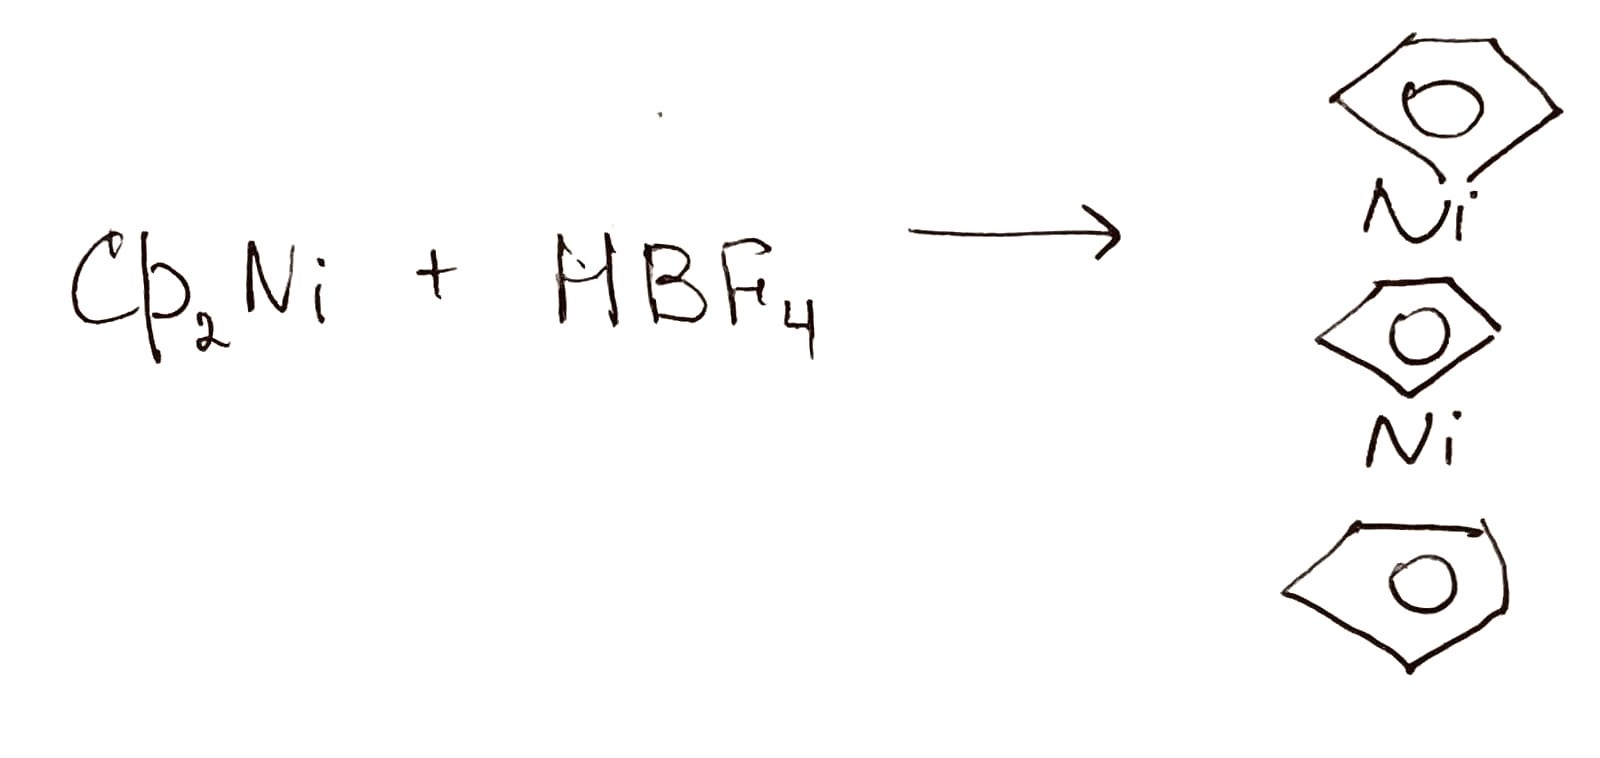
\includegraphics[scale=0.17]{xx2}}
	\end{figure}
	\item Гетеролигандные
	\begin{figure} [H]
		\centering {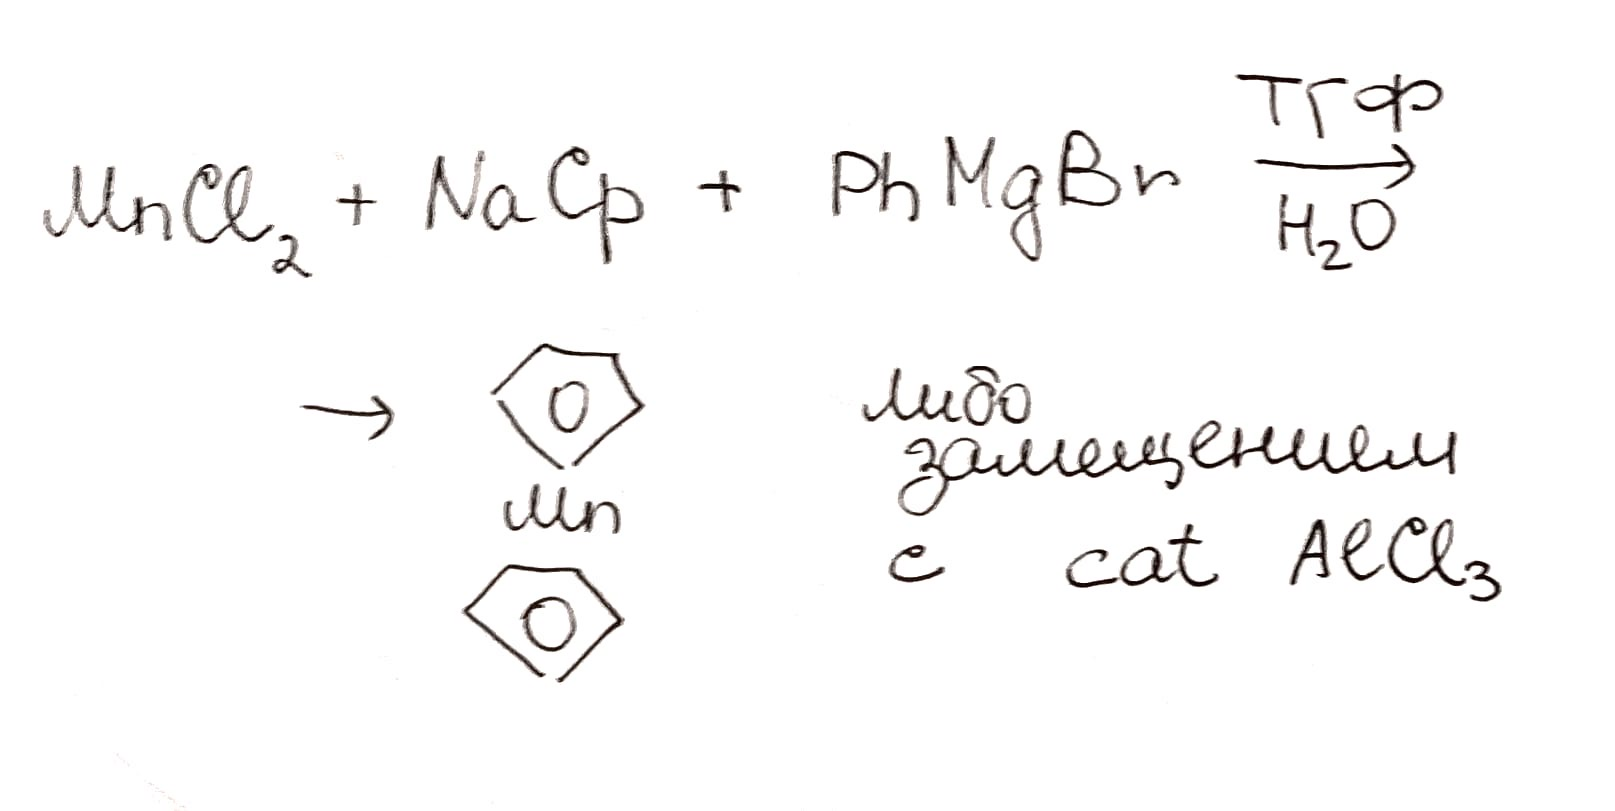
\includegraphics[scale=0.17]{xx3}}
	\end{figure}
\end{itemize}
\textbf{Условия стабильности:}\\
Правило Сиджвика не выполняется, но наиболее устойчивы те, у которых 18 электронов (нет электронов на разрыхляющих орбиталях). \\
\textbf{Геометрия:}\\
\begin{figure} [H]
	\centering {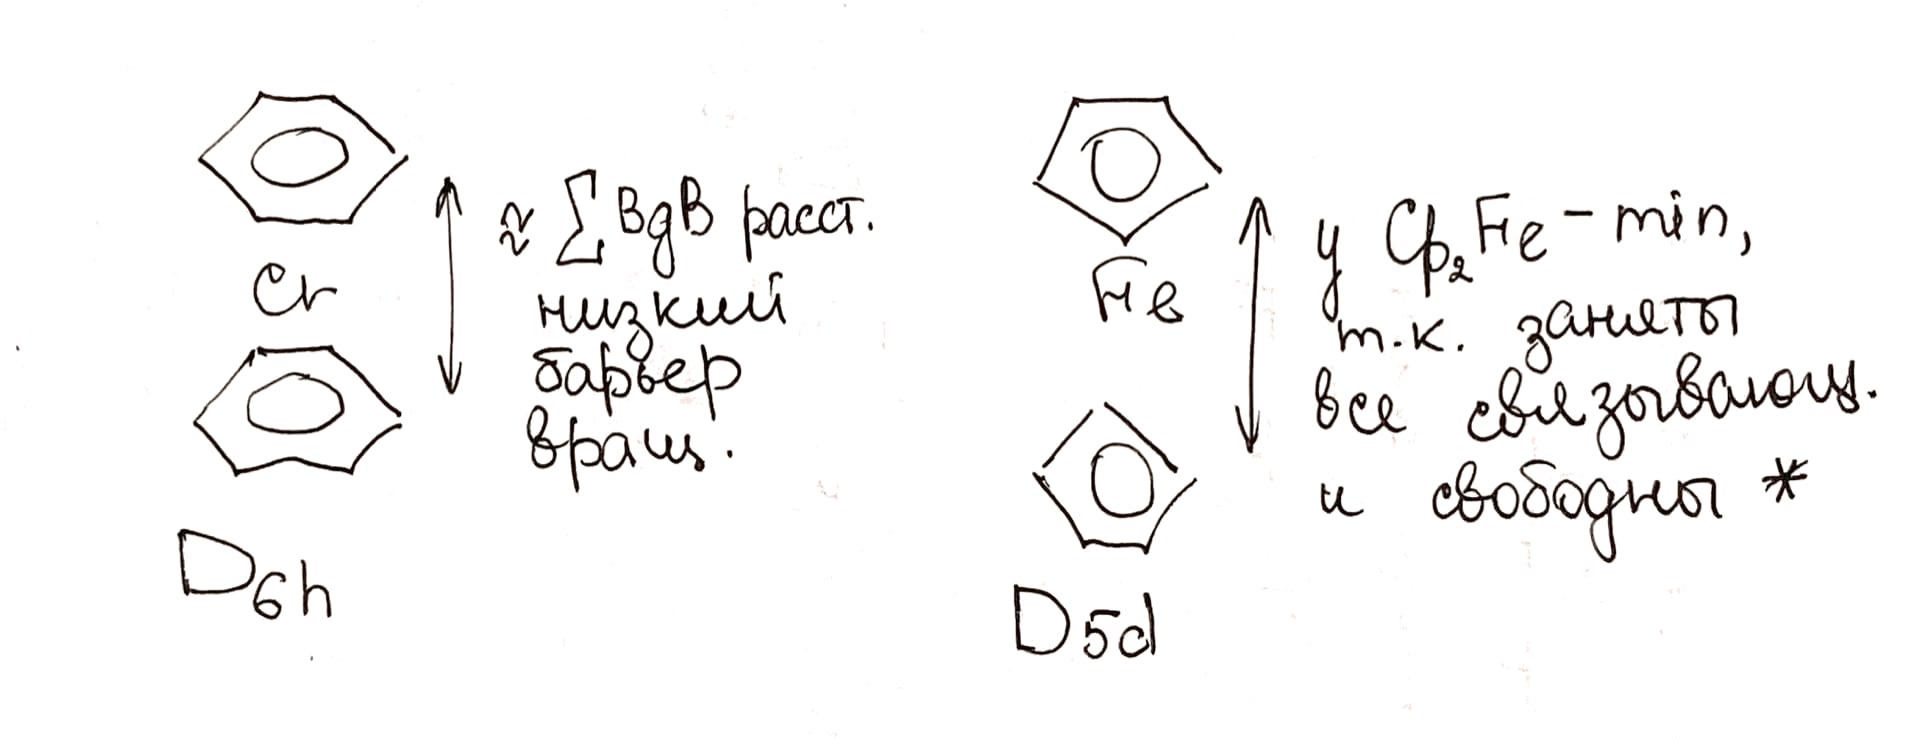
\includegraphics[scale=0.17]{xx4}}
\end{figure}
\textbf{Электронное строение (МО):}\\
\begin{figure} [H]
	\centering {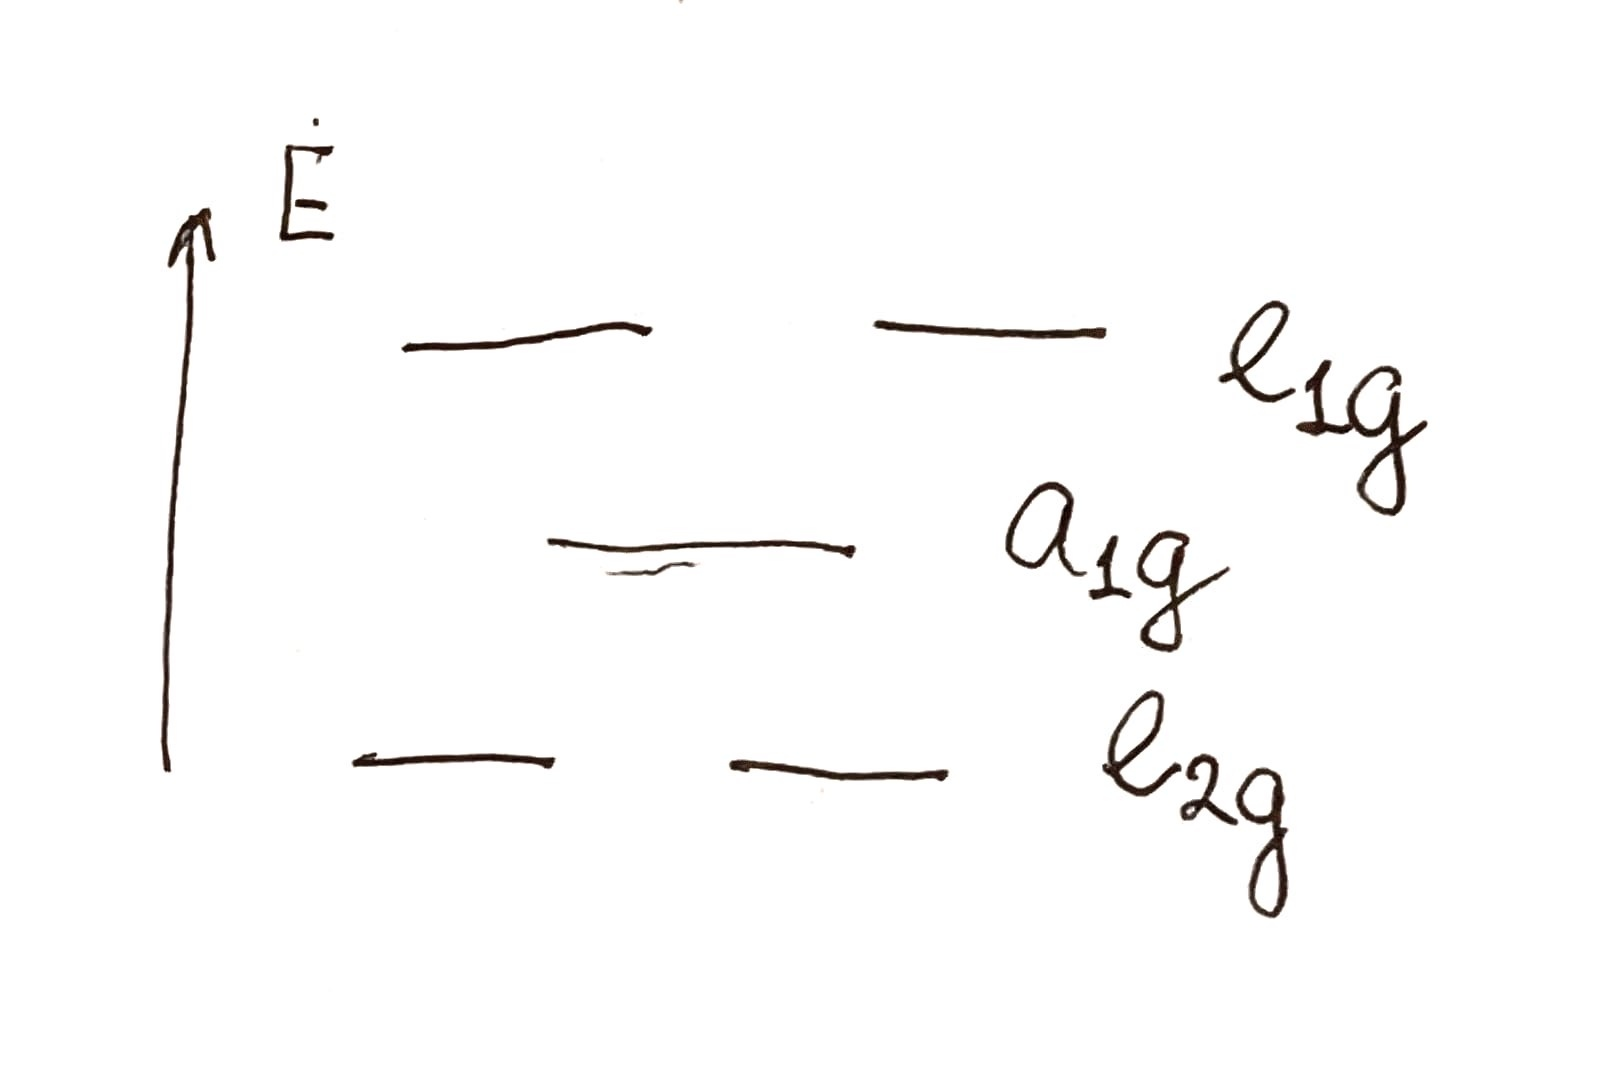
\includegraphics[scale=0.17]{xx5}}
\end{figure}
В дибензолхроме больше обратное донирование, орбитали лежат ближе по $E$ 
\textbf{Свойства:}\\
\begin{itemize}
	\item Если не 18 электронов, могут окислятся и восстанавливаться:
	\[
	Cp_2Co = -e = Cp_2Co^{+}
	\]
	\item $S_{E_{Ar}}$ (Фридель-Крафтс, металлирование)
	\item Протонирование:
	\begin{figure} [H]
		\centering {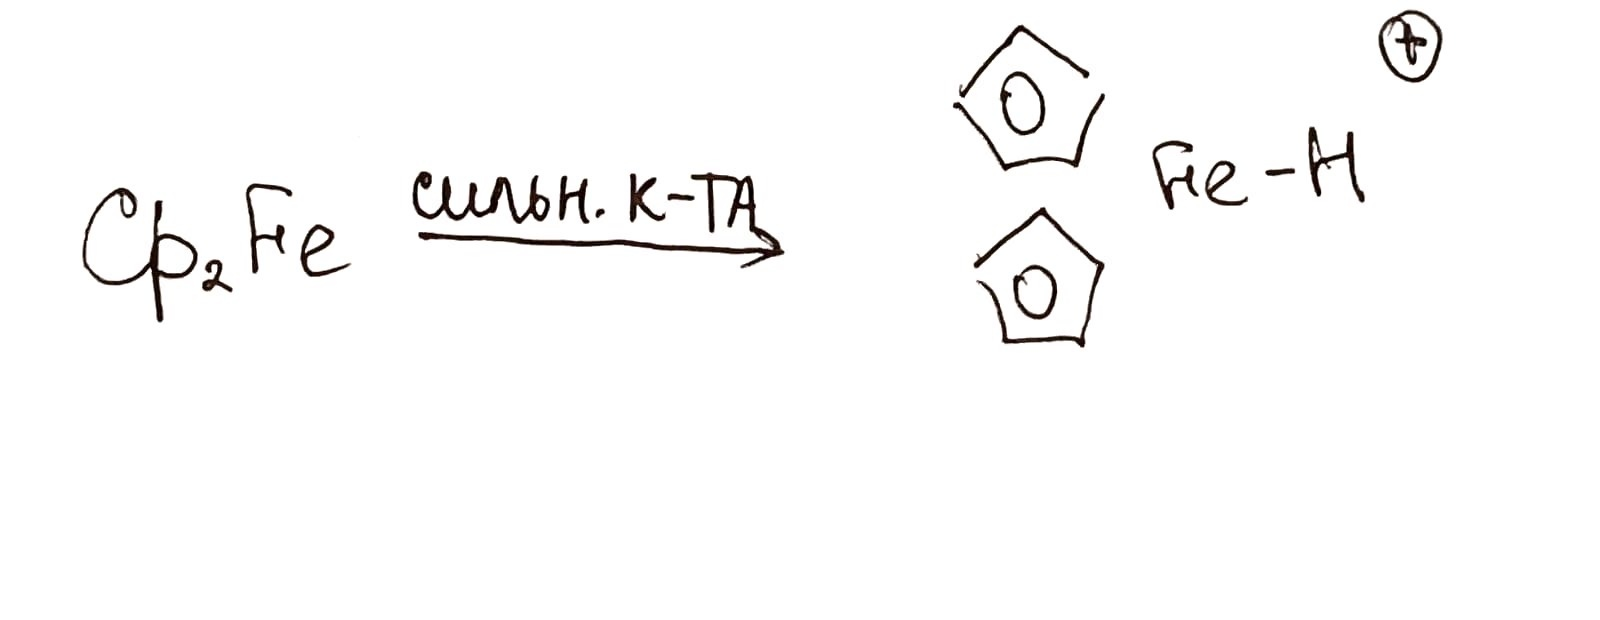
\includegraphics[scale=0.17]{xx6}}
	\end{figure}
	\item Если не 18 электронов, могут изменять гаптичность
\end{itemize}


\section*{1.28 Клиновидные сэндвичевые соединения переходных металлов (гомолигандные, гетеролигандные). Способы получения и условия стабильности, геометрия, электронное строение, свойства.}
\begin{figure} [H]
	\centering {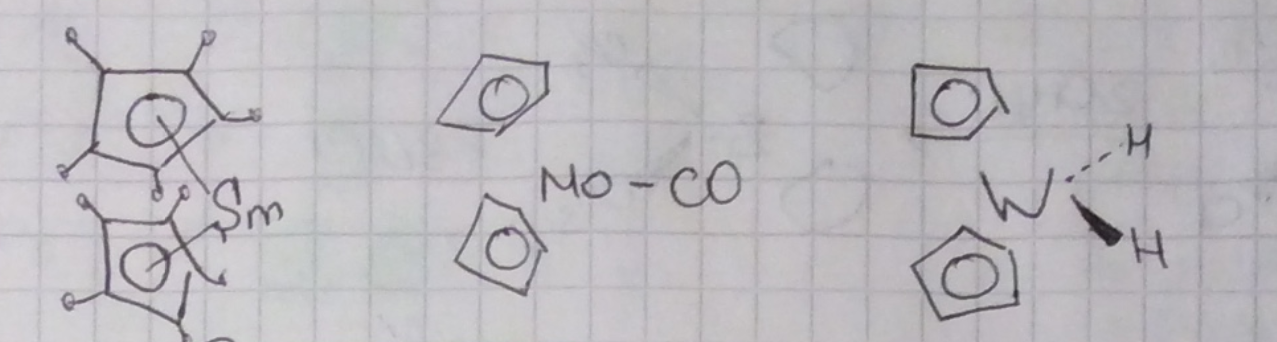
\includegraphics[scale=0.6]{ss1}}
\end{figure}
С объемными $M$, с дополнительными лигандами $(-H, -CO, ...)$
\textbf{Способы получения:}\\
\begin{figure} [H]
	\centering {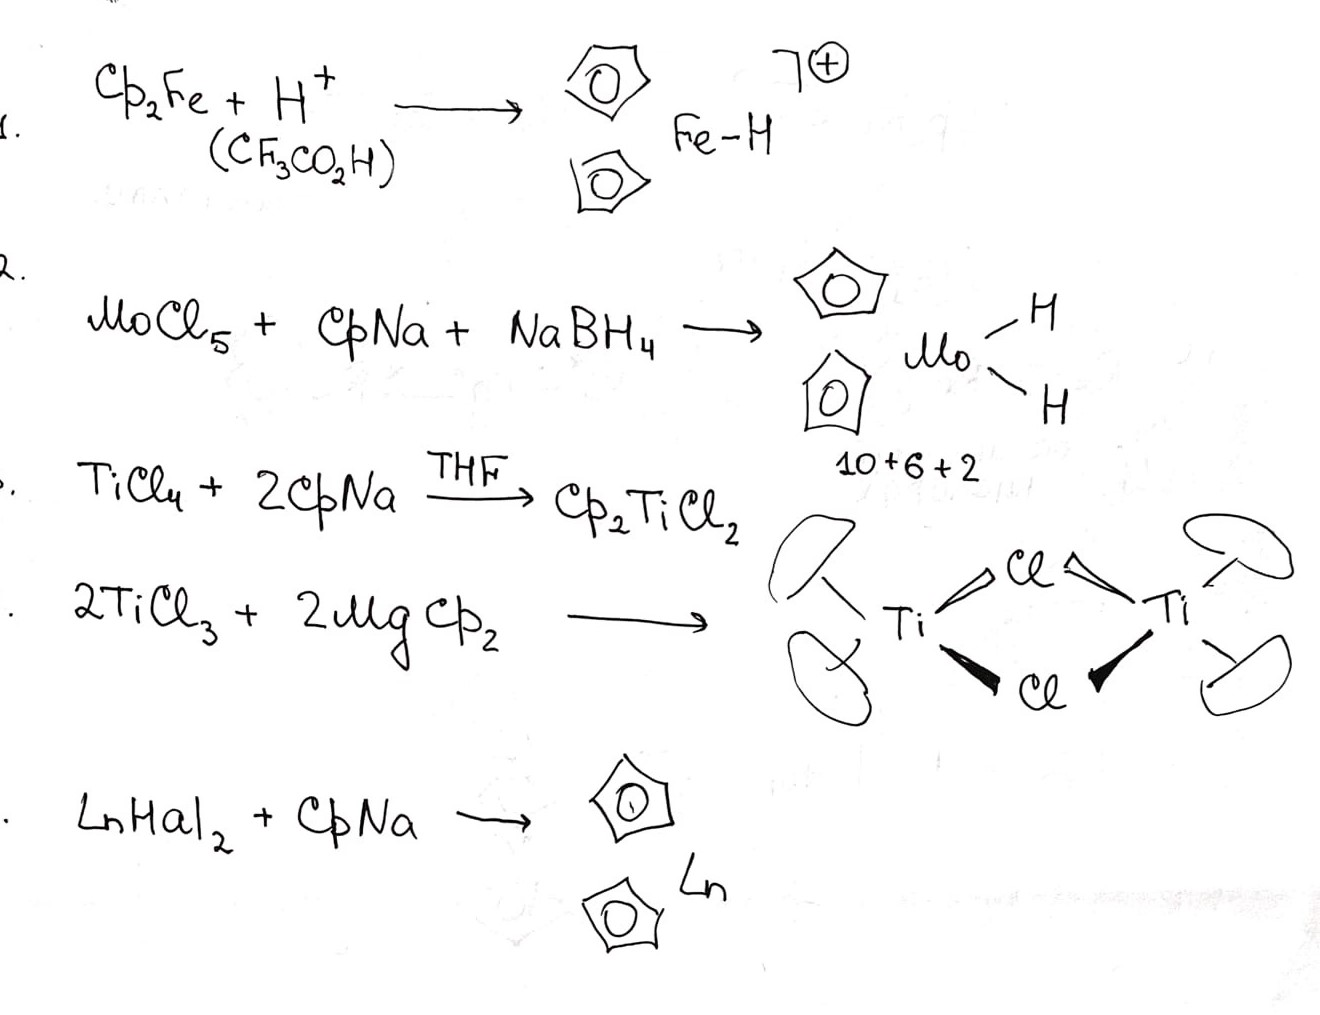
\includegraphics[scale=0.4]{ss2}}
\end{figure}
\textbf{Условия стабильности}\\
18 электронов \\
\textbf{Свойства}\\
\begin{figure} [H]
	\centering {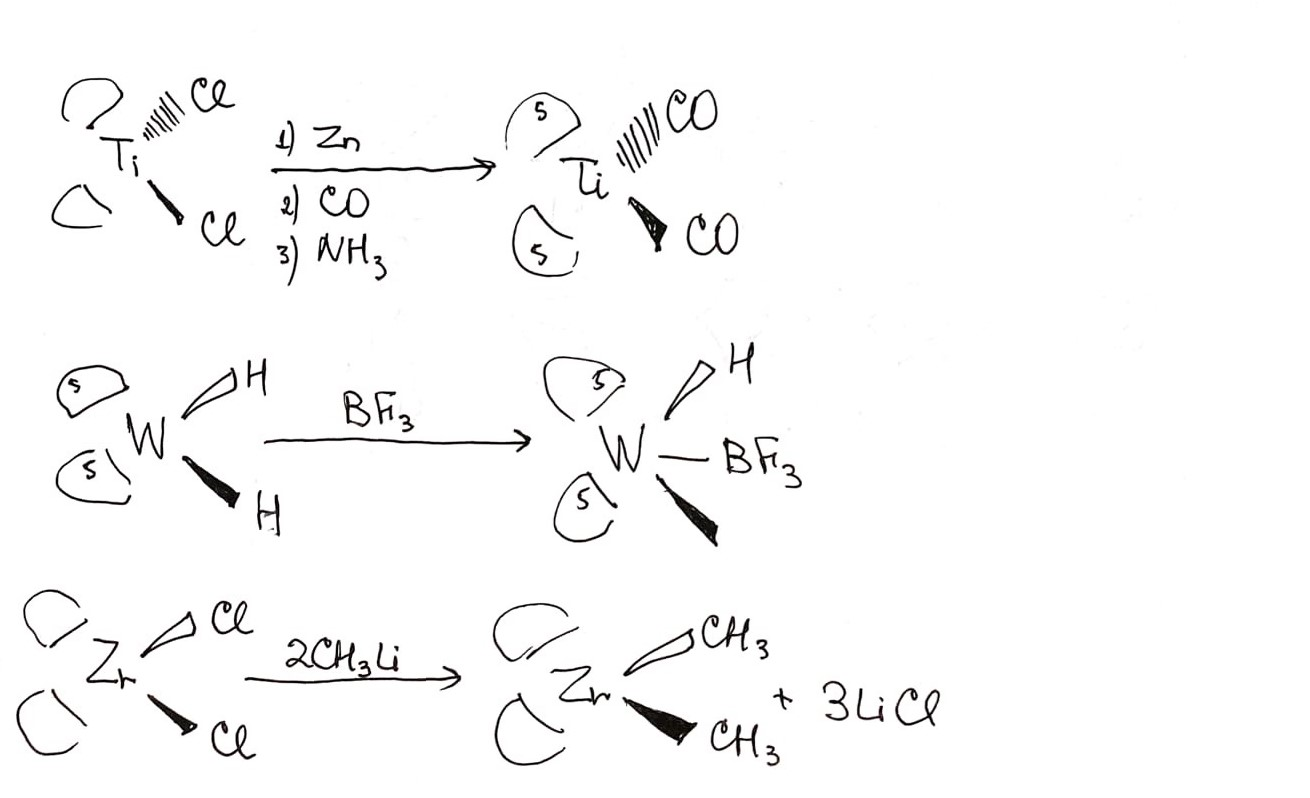
\includegraphics[scale=0.4]{ss3}}
\end{figure}

\section*{1.29 Карбонильные комплексы переходных металлов. Способы получения и условия стабильности, геометрия, электронное строение,свойства. Сравнение карбонилов различных металлов между собой.}
\textbf{Получение}\\
\begin{itemize}
	\item Металл $+ CO$:
	\[
	Ni + 4CO = Ni(CO)_4
	\]
	\item Соль металла + восстановитель + $CO$:
	\[
	CrCl_3 + Al + 6CO = AlCl_3 = Cr(CO)_6 + AlCl_3
	\]
	\item Экзотика: 
	\[
	2Fe(CO)_5 = h\nu = Fe_2(CO)_9 + CO
	\]
\end{itemize}
\textbf{Условия стабильности}\\
Правило 18 электронов \\
\textbf{Геометрия}\\
\begin{figure} [H]
	\centering {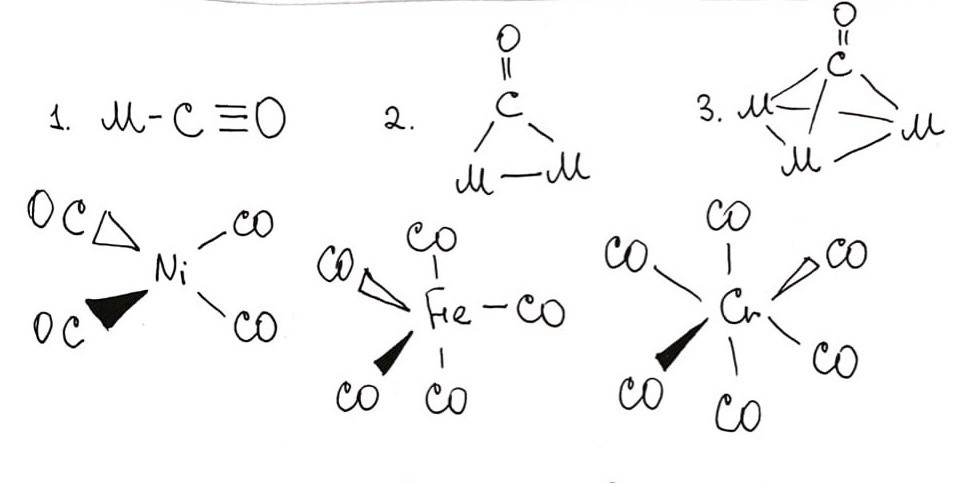
\includegraphics[scale=0.4]{dd2}}
\end{figure}
\begin{itemize}
	\item Различные полиэдры
	\item Возможно с мостиковыми лигандами и связями $M-M$
\end{itemize}
\begin{figure} [H]
	\centering {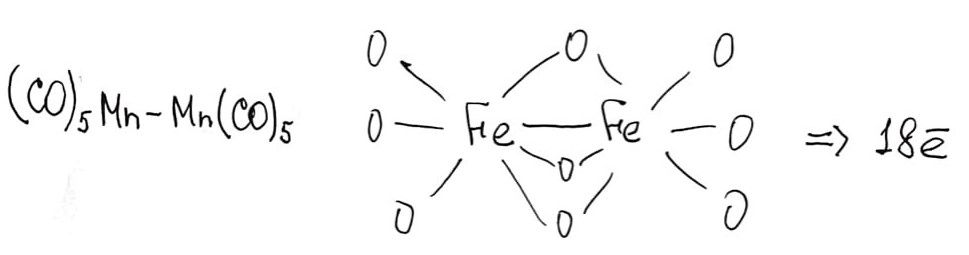
\includegraphics[scale=0.4]{dd3}}
\end{figure}
Чем ниже по группе, тем меньше вероятность мостиков. \\
\textbf{Электронное строение}\\
$\left[ M-C\equiv O \leftrightarrow M = C = O ) \right]$ \\
\begin{figure} [H]
	\centering {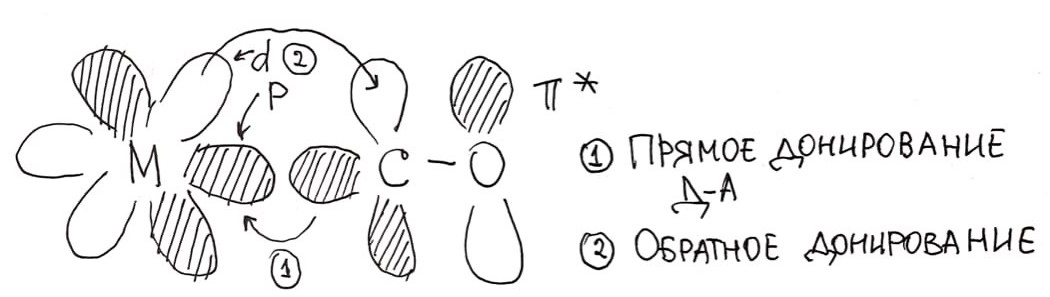
\includegraphics[scale=0.4]{dd4}}
\end{figure}
\textbf{Свойства}\\
\begin{itemize}
	\item Замещение
	\[
	Cr(CO)_6 + NR_3 = P_3NCr(CO)_5 + CO
	\]
	\item $\rightarrow $ анион
	\[
	Fe(CO)_5 = Na/Hg = Na_2^{+} \left[Fe(CO)_4 \right]^{2-}
 	\]
	\item $Nu$-атака по $CO$
	\[
	Fe(CO)_5 + NaOH = Na \left[ HFe(CO)_4 \right]
	\]
\end{itemize}
\textbf{Сравнение}\\
У $Sc$ и $Cu$ нет карбонильных комплексов, т.к. $d$-орбиталь лежит слишком высоко/слишком низко по энергии, $Ti(CO)_7$ не существует из-за стерического эффекта, у $V(CO)_6$ - $17$ электронов, у $Mn, Co$ - димеры ($Mn_2(CO)_{10}, Co_2(CO)_8$) 



\section*{1.30 Гидридные комплексы переходных металлов. Способы получения и условия стабильности, геометрия, электронное строение, свойства.}
Водородные лиганды у переходных металлов традиционно и практически исключительно называют "гидридами" независимо от того, проявляются в их поведении гидридные свойства или нет (как мы увидим в дальнейшем, многие из этих "гидридов" являются довольно сильными кислотами). \\
Гидриды могут либо быть лигандами у одного атома металла (терминальные гидриды), либо служить мостиками между двумя или тремя атомами металла, либо занимать положение внутри клетки из атомов металла.  \\
Как правило, гидридные лиганды занимают обычные координационные места, т.е. они являются "стереохимически активными". \\
В качестве доказательства наиболее часто ссылаются на структуру $HMn(CO)_5$, длина связи $H-Mn$ составляет $1,60$ ангстрем, что равно сумме ковалентных радиусов $H$ и $M(I)$. \\
Связь $M-H$ прочнее $M-C$, первая лежит в пределах $190-250$ кДж/моль, а вторая -- $150-180 $ кДж/моль  	
\begin{figure} [H]
	\centering {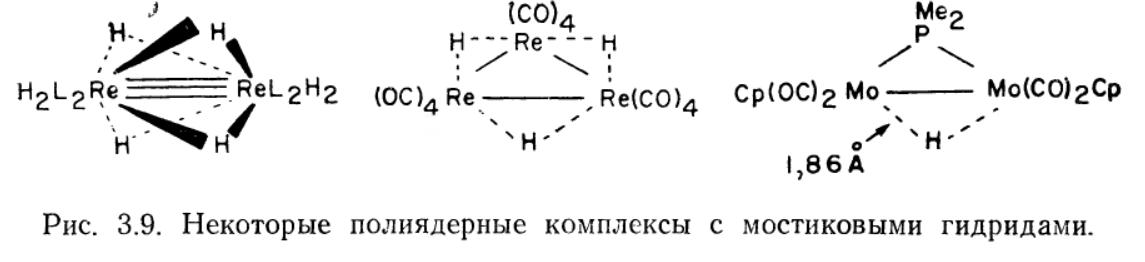
\includegraphics[scale=0.7]{oo2}}
\end{figure}
Система $M(\mu H)M$ всегда нелинейна, т.е. водород никогда не лежит на линии связи $M - M$. Такая геометрия обусловлена замкнутой трехцентровой двухэлектронной связью, поэтому расстояние $M - M$ в таких системах больше, чем в простой двухцентровой двухэлектронной связи металл-металл.
\begin{figure} [H]
	\centering {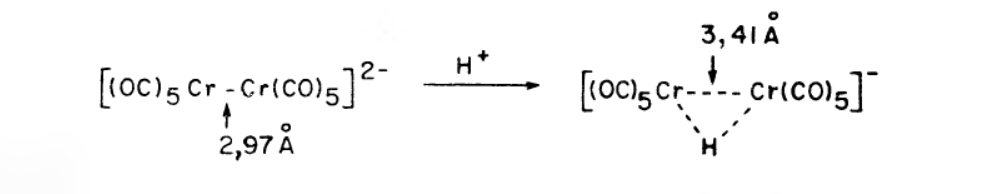
\includegraphics[scale=0.7]{oo3}}
\end{figure}
\textbf{Синтез}
\begin{itemize}
	\item Реакция окислительного присоединения $H_2$ к координационно ненасыщенным комплексам
	\begin{figure} [H]
		\centering {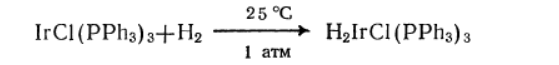
\includegraphics[scale=0.7]{oo4}}
	\end{figure}
	\item Реакция окислительного присоединения $H_2$ к координационно насыщенным комплексам
	\begin{figure} [H]
		\centering {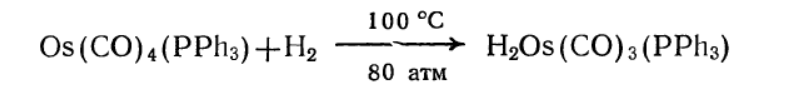
\includegraphics[scale=0.7]{oo5}}
	\end{figure}	
	\item Восстановлением в токе водорода
	\begin{figure} [H]
		\centering {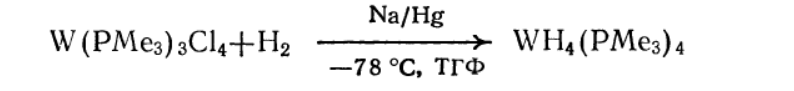
\includegraphics[scale=0.7]{oo6}}
	\end{figure}
	\item (некоторые) Гетеролиз $H_2$
	\begin{figure} [H]
		\centering {\includegraphics[scale=0.7]{oo7}}
	\end{figure}
	\item Гидрогенолиз связи металл-алкил
	\begin{figure} [H]
		\centering {\includegraphics[scale=0.7]{oo8}}
	\end{figure}
	\item Гидрогенолиз одинарных связей металл-металл
	\begin{figure} [H]
		\centering {\includegraphics[scale=0.7]{oo9}}
	\end{figure}
	\item Гидрогенолиз двойных связей металл-металл
	\begin{figure} [H]
		\centering {\includegraphics[scale=0.7]{oo10}}
	\end{figure}
\end{itemize}
\textbf{Кислотность гидридов:} \\
$HCo(CO)_4$ - намного более слабая кислота, чем хлорная, несколько более слабая, чем $HBr$ и $H_2SO_4$, и примерно такойже силы, как $HCl$ и  $HNO_3$. $H_2Fe(CO)_4$ имеет $pK_a - 4,0$ по первой ступени.
\begin{figure} [H]
	\centering {\includegraphics[scale=0.7]{oo11}}
\end{figure}
\begin{figure} [H]
	\centering {\includegraphics[scale=0.7]{oo12}}
\end{figure}
\textbf{Cвойства:} 
\begin{itemize}
	\item Диссоциация
	\[
	HMn(CO)_5 \leftrightarrows H^+ + Mn(CO)_5^-
	\]
	\item Внедрение $CO_2$
	\[
	HCr^-(CO)_5 = (CO)_5Cr - O - C(=O) - H
	\]
	\item Дейтерирование
	\[
	HCr^-(CO)_5 + MeOD = D- Cr(CO)_5
	\] 
	\item Хлорирование
	\[
	P - C(=O) - Cl + HCr^-(CO)_5 = Cl - Cr^-(CO)_5
	\]
\end{itemize}

\section*{1.31 Олефинкарбонильные комплексы переходных металлов. Способы получения и условия стабильности, геометрия, электронное строение, свойства. Сравнение параметров связи металл-олефин для различных металлов.	}

\section*{1.32 Карбонилгалогениды и карбонилат-анионы. Способы получения и условия стабильности, геометрия, электронное строение, свойства.}

\section*{1.33 Соединения со связью металл-металл, кластеры. Природа связи, геометрия молекул. Способы получения, химическое поведение.}
Определение по Коттону: \noindent \\
Кластеры — это соединения, которые содержат ограниченное число атомов металлов, которые связаны ковалентными связями друг с другом полностью или в значительной степени, даже если имеются дополнительно атомы неметаллов (лиганды), связанные с кластером. \\ \\
Для того, чтобы была связь $M_M$ необходимы:
\begin{itemize}
	\item Низкая степень окисления
	\item Большой атомный номер
\end{itemize}
Большие выступающие орбитали металла будут хорошо перекрываться. \\
Связи $M-M$ слабые по энергии, бывают одинарные и кратные\\
\begin{figure} [H]
	\centering {\includegraphics[scale=0.15]{ff2}}
\end{figure}
\textbf{Геометрия молекул}\\
Различные полиэдры, основные типы:
\begin{figure} [H]
	\centering {\includegraphics[scale=0.15]{ff1}}
\end{figure}
Правила Уэйда позволяют связать геометрию кластера с его электронным строением. \\
Принцип изолобальности: одинаковые характеристики граничных орбиталей, симметрия, число электронов, энергия \\
\begin{figure} [H]
	\centering {\includegraphics[scale=0.15]{ff3}}
\end{figure}
Определенное число электронов $\Rightarrow$ определенная геометрия \\
\textbf{Получение и свойства}
\begin{itemize}
	\item $Co(CO)_4 + AgNO_3 = (AgCo(CO)_4)_4 $
	\item $ Ru_3(CO)_{12} + \left[ Fe(CO)_4 \right]^{2-} = H^+ = H_2FeRu_3(CO)_{13} $
	\item $Os_3(CO)_{12} = t = Os_5(CO)_{16} + Os_6(CO)_{18} + Os_7(CO)_{21} ... $
	\item $ Fe(CO)_5 \rightarrow Fe_2(CO)_9 = t, HC\equiv CH = Fe_2(CO)_{15}C $ \\ имеет форму квадратной пирамиды, где в вершинах пирамиды $Fe$, а в центре основания - $C$
	\item $ Na_2Fe(CO)_4 + Fe(CO)_5 + NO^+BF_4^- = H^+ = HFe_5(CO)_{14}N $
	\begin{figure} [H]
		\centering {\includegraphics[scale=0.15]{ff4}}
	\end{figure}
\end{itemize}

